\documentclass[a4paper, 12 pt, twoside]{report}  % Comment this line out if you need a4paper
% % % % % % % % % % % Formatting preamble % % % % % % % % % % % % %

% Setting same margins on left and right pages
\usepackage[top=1.25in, bottom=1.25in,
left=1.5in, right=1.25in, twoside]{geometry}
\setlength{\oddsidemargin}{36pt}
\setlength{\evensidemargin}{36pt}

% Setting chapter heading style
%\usepackage[Bjarne]{fncychap}
%\ChTitleAsIs     
%\ChNameVar{\raggedleft\Large\rm}
%\ChNumVar{\raggedleft \bfseries\Large}
%\ChTitleVar{\raggedright \Huge\rm}

\usepackage{fancyhdr}
\usepackage{ifthen}


\renewcommand{\chaptermark}[1]{\markboth{\rm\chaptername\ \thechapter.\ #1}{}}
\renewcommand{\sectionmark}[1]{\markright{\thesection\ #1}}
\fancyhf{}

\fancyhead[LE]{\rightmark}
\fancyhead[RO]{\leftmark}


\fancyfoot[RE,RO]{\textbf{\thepage}}
\renewcommand{\headrulewidth}{0.5pt}
\renewcommand{\footrulewidth}{0.5pt}


% change plain style (eg. used on chapter pages)
\fancypagestyle{plain}{%
	\fancyhf{}
	\renewcommand{\headrulewidth}{0pt} 
	\renewcommand{\footrulewidth}{0pt} 
	\fancyfoot[CE,CO]{\textbf{\thepage}}
}

\fancypagestyle{mychapter}
{
	\fancyhf{}
	\renewcommand{\headrulewidth}{0pt} 
	\renewcommand{\footrulewidth}{0pt} 
	%\fancyfoot[CE,CO]{\textbf{\thepage}}
}

% Used for making first letter bigger
\usepackage{type1cm}
\usepackage{lettrine}
\usepackage[dvipsnames]{xcolor}

\usepackage{lipsum}

% Hyperlinks in TOC
\usepackage{hyperref}
\hypersetup{
	colorlinks=true,
	linkcolor=RoyalBlue,
	citecolor=RoyalBlue,
	urlcolor=RoyalBlue,
	linktoc=page
}

% Chaning title of TOC
\renewcommand*\contentsname{\centering\huge\textbf{Contents}}

% Generating lists of figures and tables

\usepackage{graphicx}
\graphicspath{ {figures/} }
\graphicspath{ {tables/} }
\usepackage{array}
 
\renewcommand{\listfigurename}{\huge\textbf{List of Figures}}

\renewcommand{\listtablename}{\huge\textbf{List of Tables}}

% % % % % % % % % % % % % % % % % % % % % % % % %
\usepackage{amsmath}
\usepackage{SIunits}
\usepackage{graphicx}
\usepackage{breqn}
\usepackage{floatrow}
\floatsetup[table]{capposition=top}
%\usepackage[table]{xcolor}
\usepackage{tabularx}
\usepackage{sidecap}
\usepackage{wrapfig}
\usepackage[toc,page]{appendix}
\usepackage[toc]{glossaries}
\usepackage{setspace}
\usepackage{pdfpages}
\usepackage{subfigure}
\usepackage{placeins}
\usepackage{soul}
\usepackage{SIunits}
\usepackage{amsmath,graphicx}
\usepackage{breqn}
\usepackage{multicol}
\usepackage{rotating}
\usepackage{booktabs,bm}
\usepackage{rotating}
\usepackage{verbatim, placeins}
\usepackage{stackengine,bm,accents}
\def\delequal{\mathrel{\ensurestackMath{\stackon[1pt]{=}{\scriptstyle\Delta}}}}
\newcommand{\overbar}[1]{\mkern 5mu\overline{\mkern-5mu#1\mkern-5mu}\mkern 5mu}
%\renewcommand{\thesection}{\arabic{section}}


\begin{document}
% % % % % % % % % % % front matter % % % % % % % % % % %
%\input{./chapters/cover/cover.tex}
%
% % % % % % % % % % % main matter % % % % % % % % % % % % 
\pagestyle{fancy}
\pagenumbering{arabic}
\setcounter{page}{1}

	\chapter{Introduction}

\subsubsection{Problems and Objectives of the study}

Neurons in the visual system show feature selectivity; they respond optimally to features of stimuli such as the orientation of the stimulus, the 
Over the years, sub-cortical orientation biases have been shown to play a significant role in  two key areas of study in the primary visual cortex. The first is its role in generating sharp orientation selectivity in the cortex and second is its role in generating the cortical architecture. In my thesis, I aim to further characterise the sub-cortical orientation biases and examine their role in visual processing. In the first part of my thesis, I would like to characterise the origin of the biased sub-cortical input to the cortex. There is debate as to exactly when in visual processing the orientation bias observed in the cortical input is generated. Some studies claim that this orientation bias is generated early on in the visual processing: namely the retina. Some others claim that these biases are generated through a mechanism such as excitatory convergence in the cortex. This part probes this question in two ways. 

\subsubsection{Chapter 6}

This chapter examines if there is a preponderance of a particular orientation in the cortical inputs. If the orientation bias in the cortical input is generated by Hubel and Wiesel type excitatory convergence --- where circular LGN receptive fields converge on to a V1 neuron --- we would expect that inputs to the cortex don't show any preferences (i.e. the orientations of the inputs will be randomly distributed.). Many studies however, have shown that RGCs and LGN neurons are preferentially tuned to the radial orientation (the orientation of the line joining the center of the receptive field to the centre of visual field). If the orientation bias in the inputs is derived from the retina instead, then this 
	
	
%	\chapter{Literature Review}

\section{Visual Pathways}

\subsection{Superior Colliculus}


\subsubsection{Functional Organisation of the Superior colliculus}

The superior colliculus has two major functional subdivisions. The superficial layers are primarily associated with form perception while the intermediate and deeper layers are associated with eye movements (especially generating saccades)and orienting behaviour. Studies where the superficial layers of the superior colliculus were lesioned, researchers found that animals lost the ability to discriminate between stimuli whereas lesioning the deeper layers also significantly impaired animals' ability to orient to a stimulus (cats; macaques; shrews; Casagrande, 1972). Though both the superficial layers and the deep layers of the superior colliculus perform important functions, as this thesis only focuses on the visual pathways, the organisation of the superficial layers of the SC and their receptive field properties are discussed in further detail.

The superficial SC is further subdivded into three sub-layers. The outermost of these layers is the stratum zonale. This layer consists mostly of fibres. Just below the SZ is the stratum griseum superficiale (SGS). In macaques and tree shrews, the SGS is further differentiated into upper (uSGS) and lower(lSGS). In cats, uSGS has layers 1 and 2. Just below the SGS is the final layer of the SGS, the stratum opticum or SO. The SZ, SGS and SO together form the superficial Superior Colliculus and projections to and from the visual regions of the brain (retinal, cortical and brainstem regions) terminate in this regions \cite{Swisher2010}.
\subsubsection{Connections of the Superior Colliculus}


\subsubsection{Receptive Field Properties of the superficial Superior Colliculus}

The most salient properties of the receptive fields of superior layers of the superior colliculus reported in the literature are binocularity and direction selectivity. Due to an almost complete decussation of retinal inputs to the superior colliculus, most SGS neurons receive inputs from the contralateral eye only. As a result, in most species, the binocularity of the cells has been attributed to cortical feedback. Similarly, the direction selectivity of superior colliculus has also been attributed to cortical feedback, although the proportion of direction selective cells reported in individual species are different. For example, nearly 75\% of neurons recorded in the cats were direction selective whereas the proportion was on 10\% in the macaque superior colliculus. In the tree shrew superior colliculus almost no cells are reported as direction selective, reflecting the lack of direction selectivity reported in the tree shrew cortex, further supporting the theory that direction selectivity reported in the SC are derived from the cortical neurons. Lesion studies have also reported that ablating the primary visual cortex in cats abolishes both binocularity and direction selectivity in the superficial layers of the superior colliculus.

Most superior colliculus neurons receive inputs from Y and Z cells. In cats and macaques, the superior colliculus neurons are not tuned to orientation. There are a few neurons in the tree shrew that are said to be tuned to orientation. They have large receptive fields.

\subsection{Orientation Anisotropies in the primary visual cortex}

Sasaki et al 2006
'A link between orientation selectivity and cortical retinotopy which has previously been considered independent'
Higher contrast sensitivity for the radial orientation bias in the periphery
A more global radial orientation bias- based on the quadrants
Psychophysics-they show that there is an interaction between orientation and location. There is still as higher activation for the horizontal and vertical orientations but also because the are radial?

They did test in a little bit of a greater detail by testing orientation bias near the horizontal and vertical meridians. But we have exact retinotopic location for receptive fields - Account for jitter?
Also tested for oblique locations- Then found activation in strips

Retinotopically limited stimulus

Differences: We have better spatial resolution. OI, Filtered

	Something about visuotopical organisation- being able to generate local properties from global organisation properties See Alexander et al 2004
	Ability to pool across long range receptive field connections?
	
	local organisation from global organisation of non- retinotopic settings- no not really. This was pre on-off stuff
	
Ringach 2007

Cat V1 Neurons are mostly contra dominated and Off centred.
Talks about Crair et al., 1998 who suggests that there is contralateral input which sets up the orientation columns and the ipsi input goes along for the ride- Idea similar to Alonso who also says that there is off input and the on goes along for the ride.

One important critique of sagar's model is then

What if orientation columns were not really a thing? There is adaptation- neurons change their orientations. What if this plastic process was ongoing? Just by measuring it, are we changing what is there?



Difference between the time course and spatial resolution.

Difference between the relationship between LFPs and multi unit activity: There isn't a relationship.



\subsection{Spatial Frequency Tuning}

\bibliographystyle{apacite}

\bibliography{Bibtex/library}


\chapter{Methods}

	\section{Experimental Animals}
		All experimental procedures were approved by the Florey Institute Animal Ethics committee and were conducted in accordance with the guidelines from the Animal Welfare Act 1992, The Animal Welfare Regulations (Vic) 1993 and the National Health \& Medical Research Council’s (NHMRC) Australian Code of Practice for the Care and Use of Animals for Scientific Purposes (8th Edition, listed as EA28 in the NHMRC Publications Online Catalogue under ‘Animal Ethics’). This study looked at the responses to visual stimuli in macaques (Macaca nemestrina) and tree shrews (Tupaia glis). The macaques were transported from the macaque colony (Monash Animal Research Platform) to the Melbourne Brain Centre (MBC) the day before the experiment and housed overnight and experimented on from the following day onwards. The tree shrews were obtained from the tree shrew colony at the MBC funded by the ARC Centre of Excellence in Integrative Brain Function. Macaque experiments typically lasted for 5 days and Tree Shrew experiments for 2 days. Data for this thesis was collected from a total of 6 macaques and 16 tree shrews.
		
	\section{Surgery and Anaesthesia}
	
		In all animals, initial anaesthesia was induced using a mixture of Ketamine (KETAMIL, Parnell Lab, Australia) and Xylazine (ILIUM XYLAZIL-20, Troy Laboratories, Australia; See table 1 for dosage). Once the animals were anaesthetised, venous cannulation was performed to help administer drugs and fluids. Following this, a tracheostomy was performed to administer artificial ventilation and anaesthesia during the experiment. Once the venous cannulation and tracheostomy were completed, the animals were mounted on a stereotaxic table in Horsley-Clarke co-ordinates. Artificial ventilation was provided using a respiratory pump (Harvard Apparatus, Massachusetts, USA) and anaesthesia was maintained using a gaseous mixture containing nitrous oxide, oxygen, carbogen and isoflurane (see table 1 for dosage). Paralysis was established and maintained using Vecuronium (NORCURON, Organon Australia Pty Ltd) administered intravenously (see table 1 for dosage). The animal's body temperature was maintained between 36 and 37 degrees using a servo controlled heating blanket. Silver electrodes were inserted into the frontal cortex and needles were placed in the skin on either side of the rib-cage to monitor EEG and ECG during the experiment. The end-tidal CO2 (between 3.6 and 3.8\%), the airway pressure (<10 mm/Hg) and core body temperature were also monitored during the experiment at regular intervals. Dosages of the various drugs used for the procedures detailed above are presented in Table 1.
		
		Using a microdrill, craniotomy was performed over the location of the primary visual cortex (V1) in macaques, and V1 and/or superior colliculus in tree shrews (SC; see table 1 for Horsley-Clarke co-ordinates). A durotomy was performed to remove the duramater, which both allowed a clear view of cortical surface for optical imaging as well as preserved the tip of the electrodes during microelectrode recordings. 
		
		The eyes of the animal were kept covered during surgery to protect the optics of the eye. Following surgery, the pupils were dilated using atropine sulphate (ATROPT 1\%, Sigma Pharmaceutical Pty Ltd, Australia) and rigid gas permeable contact lenses, matched for the curvature of the eyes, were fitted to prevent corneal drying. In the macaques and earlier tree shrew experiments, the eyes were refracted using a hand held projectoscope and corrective lenses were placed in front of the eye during the experiment. In the macaques, an artificial pupil (diameter= 4mm) was also placed in front of the eye. In later tree shrew experiments (9 animals), refraction was also performed during the experiment by showing animals sine-wave gratings of increasing spatial frequencies. The power of the lens where the spatial frequency resolution was the highest, was deemed the appropriate power. In most cases, the appropriate power was close to, if not the same as when no corrective lenses were added. As a result, corrective lenses were not used when they were not required, in order to limit any optical distortions the lenses may cause.
		
		Once recordings were completed, the experiment was terminated by administering the animal a lethal dose of pentobarbital sodium (200-300 mg, Merial Australia Pty Ltd) intravenously. The animals were then perfused intracardially using phosphate buffer solution (PB; 0.1M), the brain was fixed using a paraformaldehyde solution (PFA; 4\% Paraformaldehyde in 0.1M PB). The brain was removed and stored in a solution of 25\% sucrose (0.1M PB) for cryoprotection. The brain was later processed for histology.
		
		% insert table here
		
	\section{Electrophysiological Recordings}
	
		Single and multi-microelectrode recordings were made from the primary visual cortex (V1) and the superior colliculus of the tree shrews, and the macaque primary visual cortex as follows.
		
		\subsection{Single Electrode Recordings}
		
		A chamber was built around the opening using dental cement. Tungsten micro-electrodes (between 4 and 18 MΩ; FHC, Inc., ME, USA) were inserted into the cortex and the well was filled with with Agar solution (2\% Agar in 0.9\% Saline) for stability of recordings and protecting the cortex. The signal obtained from the microelectrode was first amplified (x 10,000 times; A-M Systems, WA, USA). An anti-aliasing filter (5000 Hz; A-M Systems) was applied to the signal and a HumBug noise eliminator (A-M Systems) was used to reduce 50 Hz line noise. Usually, this ‘raw signal’ was further filtered between 300 and 3000 Hz and the signal was digitised at 22.5 kHz using an analog to digital converter (Cambridge Electronic Design Limited, Cambridge, UK).  In some cases, the raw signal was also digitised in a separate channel for further analysis. The signal was also fed through an audio speaker and receptive field locations of the neurons were first plotted using the auditory feedback. The data was recorded and a template of the spikes was built using the Spike 2 software (CED, Cambridge, UK). Post stimulus time histograms (PSTHs) were built from the templated spikes for online analysis and the original signal was also saved for further analysis. At the end of each microelectrode track, electrolytic lesions were made by passing 6 μA of current for 6 to 7 seconds to identify the locations of the recordings.
		
		\subsection{Multielectrode Recordings}
		
		A 16 channel multi-electrode array (individual electrodes spaced 100 microns apart; Neuronexus Technologies, Ann Arbor, USA) was used to record from the macaque V1. The array was connected to a pre-amplifier (RA16PA, Tucker-Davis Technologies, USA), via a headstage (RA16CH), where the signal was amplified (x 10,000) and filtered (2.2 Hz to 7.5 kHz) and digitized at 12.5 kHz using TDT’s OpenEx software suite. Further digital filters were applied to separate the signal into an LFP stream (2.2-100 Hz) and a multi-unit stream (300-3000 Hz). These were saved for further analysis.
		
	\section{Stimuli}
	
	Stimuli were presented on a BARCO monitor (Frame rate= 80 Hz; Reference Calibrator Plus; Barco Video and Communications, Belgium). All stimuli were generated using the stimulus description language (SDL) and presented using the ViSaGe stimulus generator (VSG; Visage, Cambridge Research Systems, UK). To assess the stimulus preferred orientation of a unit, moving bars of 9 different orientations (18 directions) were presented to the neuron. The eye that gave the weaker or no response was occluded. Width of the bar was usually set as the narrowest bar that could still elicit a good response. The length, polarity, contrast and speed of the moving bar were all customized to elicit the best response from the neuron. Once the orientation of the stimulus was determined, the animal was presented with sine-wave gratings to determine the spatial frequency tuning of the neuron. To obtain the spatial frequency tuning, the contrast and size of the gratings were optimised and the spatial frequency was varied in steps of 0.1 and 0.3 cycles/$^o$. This was repeated at four different orientations 45$^o$ apart.
	
	\section{Data Analysis}
	
	All single unit and multi-unit recordings were templated using the Spike 2 software to isolate neurons. Each neuron at the recording site usually has a distinct set of spike parameters (shape, duration and amplitude of the components) and the spikes that were similar (with at least 60\% overlap) were grouped together as spikes from the same neuron. For each stimulus condition, a stimulus marker was produced and exported to the spike 2 software. The spikes from a neuron and the stimulus markers for each stimulus presentation were exported to a text file and analysed using custom software in MATLAB (The Mathworks Inc, MA, USA).
	
	The spikes that followed the same stimulus were gathered and displayed in a post stimulus time histogram (PSTH) so that each PSTH displays the response of the neuron to one stimulus (eg: the response to a bar of a certain orientation). In order to build a PSTH, the spikes were grouped in 20 ms intervals and the number of spikes in each bin was divided by the bin width (in seconds) to get the firing rate of the neurons (in spikes per second or Hz). The PSTH was then convolved with a Gaussian kernel (σ = 3 bins) to get the stimulus density function (SDF, see Figure 1 for example) to account for the variation in the trial-by-trial firing rate. Further measurements were performed on the SDF to define the response of the neurons to various stimuli.
	
	The response of the neuron to bars and gratings were quantified in different ways. For a moving bar, neurons showed a peak response when the bar passed over their receptive fields. Figure \ref{fig:mb} is the SDF of a neuron to a moving bar. As the bar moves over the receptive field, a peak is observed in the SDF (one for each direction). The response of the neuron is then the maximum response at each of the peaks (shown by the red circles).
		\begin{figure}[H]
		
		\includegraphics[width=\linewidth]{methods/SDF_movingbar.jpg}
		\caption{The SDF of a neuron’s response to a vertical bar moving bidirectionally. The maximum response in each direction is highlighted with red circles}
		\label{fig:mb}
		\end{figure}

	When shown gratings, neurons respond differently. A neuron, based on whether it demonstrates linear summation over its receptive field or not, responds differently to a grating. For example, ‘linear’ cells give a response modulated to the temporal frequency of a grating (see Figure \ref{fig:fourier}a; TF= 4Hz). A Fast Fourier Transform of the SDF is taken (Figure \ref{fig:fourier}b) and the peaks observed indicate that the respective frequencies have a high magnitude in the original signal. In this case, the FFT has two distinct peaks (red circles), the first one is at 0 Hz and the second one at 4Hz. The peak at 0 Hz is the F0 component of the response and is equal to the average of the signal in figure \ref{fig:fourier}a. The second peak is the F1 component and gives the fundamental frequency of the neuron’s modulated response (4 Hz). ‘Non-linear’ cells don’t show a modulated response to gratings, especially for higher spatial frequency gratings and as a result, the only distinct peak in the FFT corresponds to the F0 component (0 Hz). 
			\begin{figure}[H]
			
			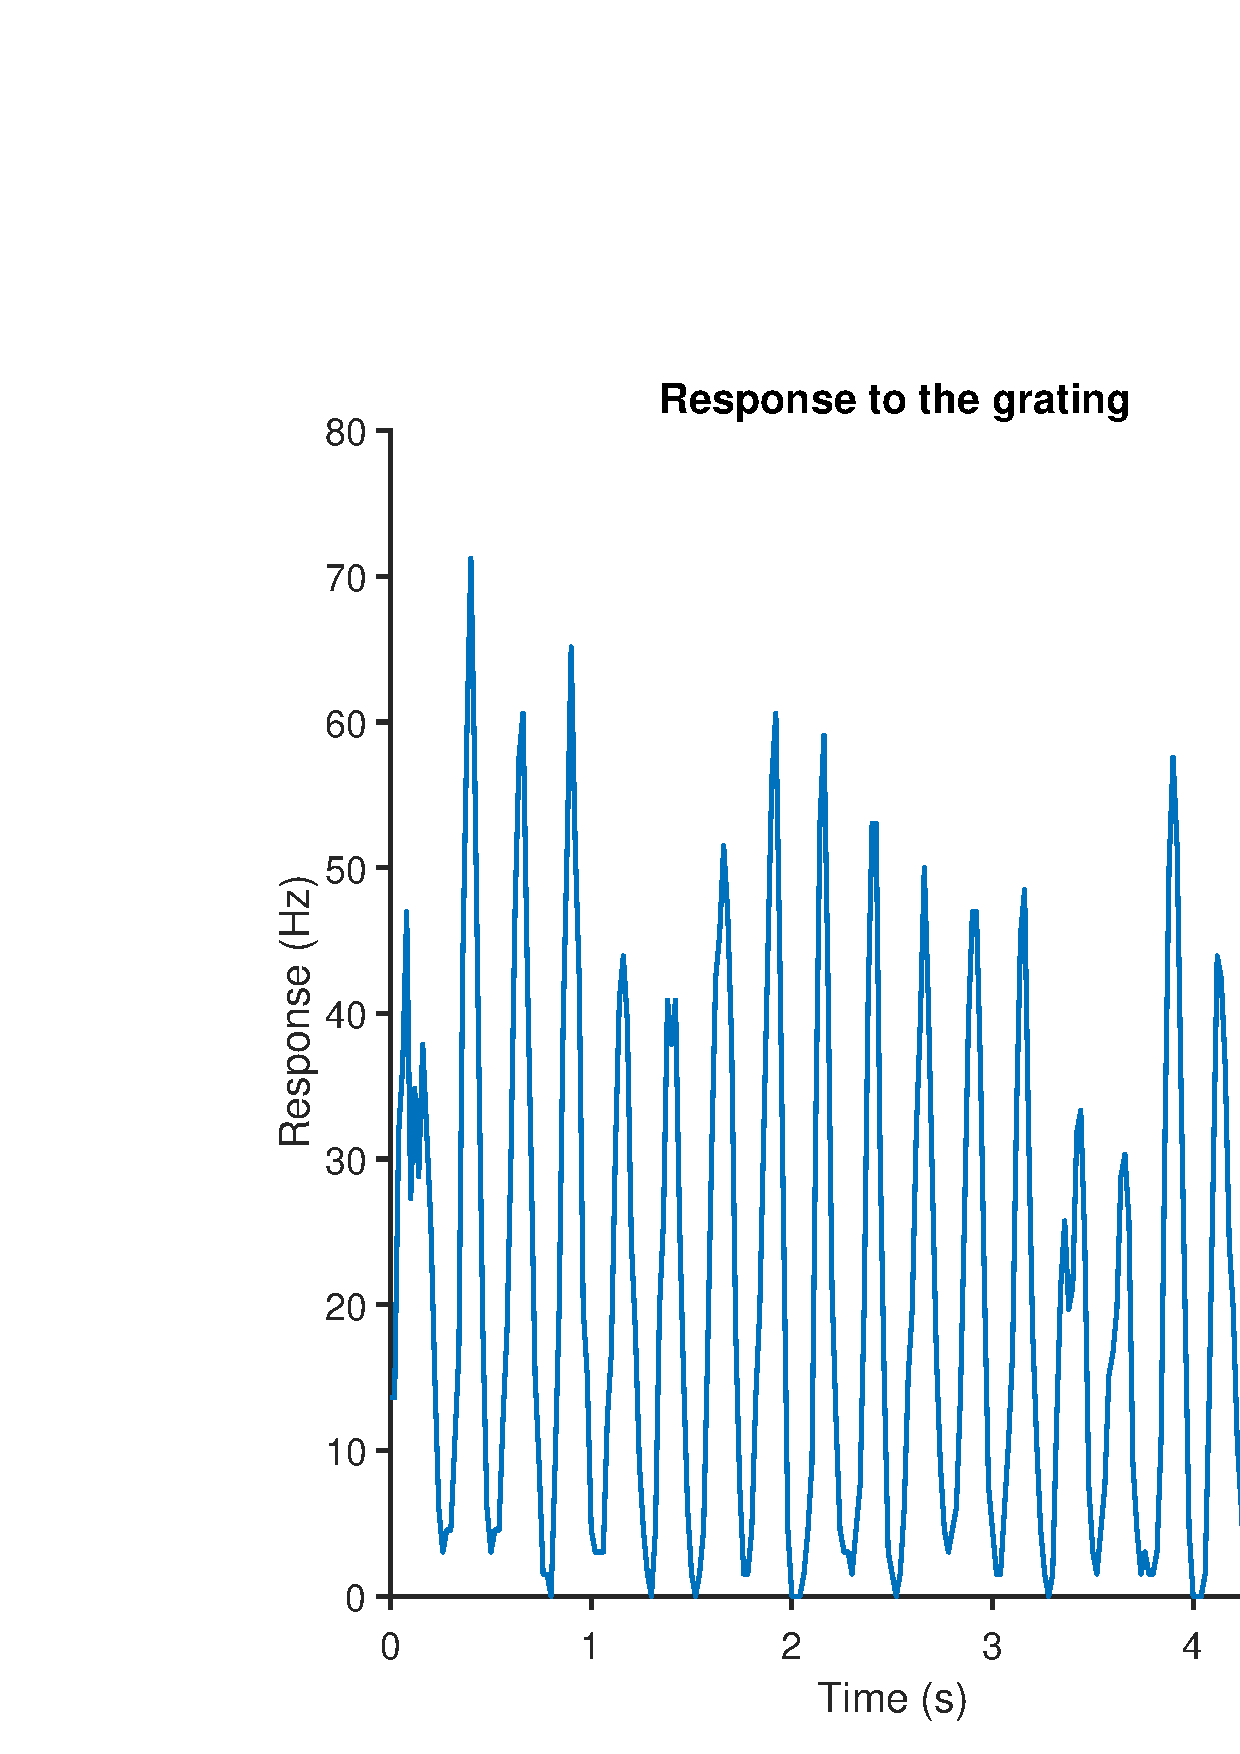
\includegraphics[width=\linewidth]{methods/Fourier.jpg}
			\caption{a) the SDF of a ‘linear’ cell. The first 4.3s was the stimulus presentation duration. A blank screen was presented for the last 0.7s. b) The fast fourier transform (FFT) of the signal in fig\ref{fig:fourier}a. There is a peak at the F0 component as well as at 4 Hz, which was also the temporal frequency of the sine wave grating.}
			\label{fig:fourier}
			\end{figure}
	
	Cells were first classified as linear or non-linear neurons – with our cortical and collicular data, comparable to the classical categories of simple and complex in the primary visual cortex (Hubel and Wiesel , 1962) and X and Y like in the lateral geniculate nucleus (Enroth-Cugell and Robson, 1966). This was done by taking the modulation index (Skottun et al., 1991) which is the ratio of the F0 and F1 components of the response. Traditionally, the modulation index is calculated by dividing the F1 component of the response by the F0 component. Neurons with modulation index less than 1 were classified as non-linear cells and cells with modulation index greater than 1.5 were classified as linear cells. Recently, a modified measure of the modulation index was proposed to measure linearity in the tree shrew primary visual cortex (Van Hooser et al., 2013). Using this measure, the range of values the modulation index could take was between 0 and 2 where neurons with modulation index less than 1 were classified as non-linear cells and where neurons with modulation ratio between 1 and 2 were classified as linear cells. This measure of modulation index was chosen to enable comparison with earlier tree shrew studies. For non-linear cells, the F0 component of the response was used for further analysis while for linear cells, the F1 component was used. From the response of the neuron to drifting sinusoidal gratings of increasing spatial frequencies, the spatial frequency tuning curves of the neuron was constructed and the peak spatial frequency and the half width at half height were calculated.
	
	\section{Histology}
	
	After the experiment, the tissue was processed for histology as follows. The brain was stored in a 25\% sucrose solution until it sank. This was to ensure that the tissue was cryoprotected. The brain was cut into blocks so that only the areas of interest were sectioned. The brain was frozen and 50 micron sections were made using a cryostat (Leica CM3050S, Leica Microsystems, Nussloch, Germany). The sections were collected and stored in a Sodium Azide solution (0.1\% in 0.1M PB) till they could be mounted on gelatinised slides after which they were dried overnight and stained.
	
	\subsection{Cresyl violet staining}
	
	First the sections were dehydrated using increasing concentrations of ethanol solution. Then, chloroform was used to de-fatten the sections. This was followed by rehydrating sections in decreasing concentrations of ethanol. The sections were then stained using Cresyl Violet Acetate solution (0.1\%, Sigma-Aldrich, Inc., USA) and differentiated using a solution of 5\% percent acetic acid in 95\% ethanol. The sections were then fixed in histolene and the slides were coverslipped.
	
	\subsection{Track Reconstruction}
	
	In order to reconstruct electrode tracks, the electrolytic lesions were located under a light microscope and digitised (Zeiss Axiocam Digital Camera, Zeiss, Germany). The shrinkage was calculated by comparing the recorded and observed distances between lesions using Adobe Illustrator(Adobe systems software Ltd). The shrinkage calculation was used to accurately determine the actual depth of the units recorded. In tree shrew V1, based on the location of the unit, it was classified as layer 4 or layer 2/3. In the shrew superior colliculus, the units were categorized as either belonging to the superficial or deeper layers of the superior colliculus.
	
	\section{Optical Imaging of Intrinsic Signals}
	
	Optical imaging of intrinsic signal is a high resolution imaging method that is used to detect the changes in blood oxygenation level in areas of neuronal activity. As a result of neuronal activity there is increased oxygen consumption in the surrounding tissue which leads to an increase in the level of de-oxy haemoglobin in the blood. This leads to a difference in reflectance in the tissue between regions where there is oxygenated and de-oxygenated blood and it is this signal that OI detects. This is the same signal as the fMRI BOLD signal but optical imaging has one key advantage over BOLD imaging. Whereas the fMRI signal has the resolution in the scale of millimetres, OI can detect  signals at at least one order of magnitude higher resolution, allowing us to visualize the organization of neuronal activity at the scale of cortical columns. So, Optical imaging was used to image the functional activity of the macaque primary visual cortex. 
	\subsection{The apparatus}
	
	In order to acquire OI maps of the primary visual cortex, first, a tandem lens macroscope was attached to a slow-scanning CCD camera. A light source is used to provide illumination for the duration of the imaging and the acquired frames were converted into a digital signal using an analog to digital converter. The specifications of these equipments are detailed below.
	
	\subsubsection{Macroscope and camera}
	
	A tandem lens macroscope was constructed by arranging two camera lenses (Pentax lenses, f= 50mm) end-to-end. This macroscope had a shallow depth of field which allowed us to focus at a specific depth below the surface of the cortex. In this manner, we acquired the blood flow changes related to the neuronal activity at the depth where the lens was focused. The macroscope was connected to a slow scan CCD camera (Teli CS 8310B; Ts’o et al., 1990) which acquired and transmitted images to the imaging system (VDAQ Imager 3001, Optical Imaging, Rochester, NY). 
	
	\subsubsection{The Chamber}
	
	As the images were acquired in-vivo in an anaesthetized macaque, there was the possibility of the image being contaminated by movement artefacts caused by the animal’s respiration and heartbeat. To reduce this, a metal chamber (diameter= 10 mm) was placed on the skull surrounding the exposed cortical area. It was sealed in place using dental cement (Dentimex VA, Netherlands) and ensured that no leaks were present. Once the chamber was fixed to the skull, it was filled with Silicone oil (Polydimethylsiloxane 200 fluid, viscosity 50 cSt, Sigma-Aldrich, Inc., USA) and sealed with a coverslip. In the macaque, due to the angle of the imaged area, we used a metal chamber without the metal pipes traditionally used to fill the chamber. The cylinder was overfilled with Silicone oil and the coverslip tightened. Where bubbles were present, the process was repeated until a clear view of the cortex was achieved.
	
	\subsubsection{The Illumination System}
	A circular fibre-optic attachment was connected to the camera lens for uniform illumination during optical imaging. First, a green light filter (545 nm) was used to obtain an image of the cortical surface with blood vessel landmarks (the green image). Then a longer wavelength (630 nm) filter was used for imaging. This wavelength of light was used because it was shown to reliably isolate the haemodynamic changes related to neuronal activity. Shorter wavelength lights (< 600 nm) reveal more of the blood volume changes while light of wavelength longer than 630 nm primarily detected light scatter effects. Light at 630 nm was the longest wavelength of light we could use to ensure maximum penetration of the light into the cortex while still imaging the haemodynamic changes.
	
	\subsection{Image acquisition}
	
	\subsubsection{Stimulus presentation}
	
	Stimulus was generated by the ViSaGe system and displayed on the BARCO monitor as described below. The Visage and the camera were synchronized by the means of an optical imaging interface (VDAQ Imager 3001, Optical Imaging, Rochester, NY). The interface started the camera when the stimulus presentation began. The stimuli were eight full field, bidirectional, square wave gratings (contrast =100\%; Spatial Frequency = 1-2.5 cycles/degree; Temporal Frequency = 1.5 Hz) of changing orientations. The stimulus was presented for 7.2 seconds, followed by a 10 second blank. This inter-stimulus interval allowed the OI signal to return to baseline. This was repeated 50 times to improve the signal-to-noise ratio.
	
	\subsubsection{Image acquisition system}
	
	The macroscope was focused below the surface of the cortex between 550 and 700 μm. Then, when the stimulus was presented, the Imager 3001 simultaneously started the camera which acquired 18 frames, each 400 ms long while the stimulus was presented. There was no image acquisition during the inter stimulus blank time. In order to get an image of the cortex at rest, a blank stimulus was presented for 7.2 s, followed by a 10 s interstimulus interval. The camera had a 14-bit bit-depth, which allowed the detection of very small variations in the OI signal. The individual frames for each block (10 trials per block) were first saved by the imaging system and exported to MATLAB for further analysis.
	
	\subsection{Analysis of Intrinsic Signals}
	
	\subsubsection{Pre-processing of the data}
	
	Prior to the analysis, the data acquired had to be corrected for luminance artefacts. We did this by averaging frame numbers 3 to 16 from all the 50 trials for each stimulus condition (between 1200 and 6800 ms) and dividing it by the average of the first frame across 50 trials. These frames were chosen as the signal from OI when using the 630 nm light is biphasic (see figure \ref{fig:oit}). The initial signal first dips below the baseline and then increases later, peaking at approximately 5 s after the stimulus was presented. This is generally consistent with the time-course of the de-oxyhaemoglobin concentration (Malonek and Grinvald, 1996). To account for the illumination effects, the first frame subtraction method was employed to create a differential map. In this method, the blank was taken as the first frame and the activity of all other frames are calculated as the difference of the frame from the ‘blank’ frame. This division by the blank is equivalent to subtracting and dividing by the blank since the optical imaging signal is relatively small (see Pouratian \& Toga, 2002).
	
		\begin{figure}[H]
		
		\includegraphics[width=\linewidth]{methods/OI_timecourse2.jpg}
		\caption{The time course of the OI haemodynamic signal for the duration of the stimulus presentation. The deoxyhaemoglobin levels briefly increase before decreasing, leading to a decrease in pixel intensity followed by an increase.}
		\label{fig:oit}
		\end{figure}
	
	\subsubsection{Obtaining single condition and orientation maps}
	
	The differential map is bandpass filtered in order to obtain the single condition map. This is done as follows. First the differential map is low pass filtered using a Gaussian kernel with a large sigma value (312.5 microns). The low pass filtered map is subtracted from the differential map to obtain the highpass filtered map which is once again filled with a Gaussian kernel with a small sigma value (100 microns). The resulting map is the single condition map (SCM; see figure 4).
	
	\begin{figure}[H]
		
		\includegraphics[width=\linewidth]{methods/filters.jpg}
		\caption{The filtering process used to generate single condition maps. The differential maps are first high-pass filtered to remove spatial scale signals and a smaller low-pass, smoothing filter was used to remove the high spatial noise.}
		\label{fig:filters}
	\end{figure}
	
	The single condition maps obtained for each orientation are then vector averaged (Swindale, 1998) to create the orientation domain map.


\chapter{Radial Bias in large spatial scale optical imaging signal in the macaque Primary Visual Cortex}

\pagebreak

	\section{Summary}
	
	Neurons in the primary visual cortex are tuned to orientation and similarly oriented neurons are arranged in columns, with orientation columns arranged like spokes around a pinwheel. The different orientations are however not equally represented. Two different types of biases have been reported in the representation of orientations in the primary visual cortex, namely the oblique effect and the radial orientation bias. Electrophysiological and fMRI studies have shown a preponderance of the radial orientation in the primary visual cortex of mammals. However, optical imaging of intrinsic signals (OI), which are related to the fMRI signals do not show this radial bias. Here, OI signals on a spatial scale comparable to that of the fMRI signals were examined. The orientation selectivity of the spatially unfiltered, raw signal obtained from OI was compared to the radial angle and a significant radial bias was found in this signal. When a similar analysis was performed on a traditionally band-pass filtered OI signal, a much weaker radial bias was found. As the OI signal is predominantly due to synaptic and pre-synaptic activity, it is proposed that the global signal in OI corresponds to cortical inputs. If the cortical inputs are biased for only a small number of orientations, then this provides evidence for a model of orientation selectivity where orientation tuning of cortical neurons are sculpted from orientation biases encoded in a small number of broadly tuned channels.
			
\pagebreak

	\section{Introduction}
	
	Neurons in the primary visual cortex are tuned to orientation and the orientation tuned neurons are organised in columns. Hubel and Wiesel (1962) showed that neurons in Area 17 of cats were sharply tuned to orientation. These neurons were also grouped into neurons of similar orientation. Optical imaging studies in the cat A17 and 18 showed that the cortical orientation columns were organised as the spokes of a pinwheel, converging on the pinwheel centre (Bonhoeffer and Grinvald, 1991; Grinvald et al., 1986). Models of orientation selectivity and cortical architecture assume that neurons are equally tuned to all line orientations. However, studies suggest that there is an overrepresentation of some orientations in the visual system. Two types of orientation biases have been demonstrated in the visual system. The first is the oblique effect, which manifests as an underrepresentation of the oblique orientations while the horizontal and vertical orientations are overrepresented (see Appelle, 1972 for review). The second is the radial bias; where neurons are preferentially tuned to the orientation parallel to the line joining the centre of the receptive field to the centre of the visual field (Levick and Thibos, 1980). Both these biases have been reported in the macaques.
	
	Where the relationship between the receptive field location and visual field locus were studied, a radial bias has been reported every time. Early studies of biases in orientation representation in the cortex reported a strong oblique effect in electrophysiological studies (Chapman and Bonhoeffer, 1998; Coppola et al., 1998; DeValois et al., 1982; Kennedy et al., 1985; Leventhal, 1983; Li et al., 2003; Mansfield, 1974; Mansfield and Ronner, 1978; Orban and Kennedy, 1981, Payne and Berman, 1983; Pettigrew et al., 1968); which was congruent to the findings of a prominent oblique effect in behavioural studies reported in most species, from humans to octopuses (Appelle, 1972; Campbell et al., 1966; Furmanski and Engel, 2000; Rovamo et al., 1982). However, these studies examined the orientation preferences of neurons without studying their corresponding receptive field locations. Later studies that characterised the receptive field location with regards to the visual field locus all reported a radial bias in almost all species that were studied using electrophysiological studies (Levick and Thibos, 1980; Levick and Thibos, 1982; Maloney et al., 2014; Passaglia et al., 2003; Leventhal, 1983; Leventhal and Schall, 1983; Smith et al., 1990; Vidyasagar and Henry, 1990; Schall et al., 1986a; Schall et al., 1986b, Shou and Leventhal, 1989), fMRI imaging studies (Sasaki et al., 2006; Swisher et al., 2010; Mannion et al., 2010) and behavioural studies where subjects observed natural scenes instead of oriented gratings (Hanson and Essock, 2004).
	
	One of the key tools that have been instrumental in revealing cortical architecture is optical imaging of intrinsic signals (OI). Using OI, not only have the ocular dominance domains and orientation domains been visualised, but their relationships with each other have also been examined (Bartfeld and Grinvald, 1992). The haemodynamic change accompanying neural activity that is recorded using OI is akin to the BOLD (Blood Oxygen Level Dependent) response observed in fMRI (Menon et al., 1995; Logothetis et al., 2001). While the orientation biases studied using the fMRI BOLD responses reveal a radial orientation bias, only the oblique effect has been reported using OI (Chapman and Bonhoeffer, 1998; Coppola et al., 1998; Grabska-Barwinska et al., 2009).
	
	One reason for this discrepancy in these findings could be due to the spatial scale at which these signals are studied. The BOLD signal has a poorer spatial resolution compared to the OI signals, which is capable of resolving cortical columns (Churchland and Sejnowksi, 1988). The BOLD and OI responses predominantly consist of the pre-synaptic and synaptic activity with the extracellular, spiking activity forming a fairly small part of the response (Logothetis et al., 2001). Traditionally, images obtained using OI are band-pass filtered to reflect activity corresponding to a narrow spatial scale (between 100-500 microns). While this spatial filtering has the advantage of isolating the weaker, smaller spatial scale spiking activity, it has the disadvantage that by omitting the larger spatial scale activity, any information present at this spatial scale is lost. Here, we aimed to use the unfiltered larger spatial scale signal. We hypothesised that when this larger spatial scale signal is studied in the anaesthetised macaque striate cortex, we will find a bias for the radial orientation as has been reported in the fMRI studies. 
	
		
	\pagebreak
		
	\section{Methods}
	In this study, we imaged and recorded from the cortex of five, anaesthetised male macaques (Macaca nemestrina, 2-4 years old). All experimental procedures were approved by the Florey Institute of Neuroscience and Mental Health Animal ethics committee and conformed to the guidelines of the National Health and Medical Research Council’s Australian Code of Practice for the Care and Use of Animals for Scientific purposes.
		\subsubsection{Surgery and anaesthesia}
		Surgical procedures were as described in the methods section. Briefly, animals were anaesthetised using a Ketamine/Xylazine mixture (Ketamil, 15mg/kg, i.m., Parnell Laboratories, Australia; Cylazil, 2mg/kg, i.m., Troy Laboratories, Australia). Venous cannulation was performed on the cephalic vein to administer fluids and paralysant (Norcuron, initial bolus of 0.7 mg/kg followed by 0.2 mg/kg/hr, Organon Australia Pty Ltd) to the animal and a tracheostomy was performed to administer the anaesthesia (0.5-2\% Isoflurane in a mixture of nitrous oxide and oxygen (70:30)) during the experiment. The animal was placed in a stereotaxic frame and its head fixed using ear bars. During the experiment, the end-tidal CO2 (3.6-3.8\%), electrocardiogram, electroencephalogram and the core body temperature were all monitored. A craniotomy and durotomy were conducted over the location of the primary visual cortex (Horsley-Clarke co-ordinates: 24-34 mm posterior and 2-10mm lateral). The eyes were dilated by applying 0.1\% Atropine (Sigma Pharmaceuticals Pty Ltd, Australia) and rigid, gas permeable lens were introduced to prevent corneal drying and optical lenses and artificial pupil (4mm) were used to correct any refractive errors and reduce optical aberrations.
	
		\subsubsection{Optical Imaging of Intrinsic Signals}
		
		\paragraph{Setup}
		Optical imaging of intrinsic signals was used to obtain the haemodynamic change related to the neural response to orientation stimuli. The OI setup involved two camera lenses (2 x Pentax lenses, f=50 mm) arranged in a tandem fashion (Frostig et al., 1990) connected to a CCD camera (Teli CS8310B). The tandem lens arrangement allowed us to choose a narrow plane of focus. An LED light source was used to illuminate the cortical surface. Before stimulus presentation, a high contrast, ‘green image’ of the surface of the cortex was obtained by illuminating the cortical surface with a green light (filter wavelength=545 nm). This provided us with cortical landmarks which were later used in determining the locations for electrode tracks of topographical recordings. Following this, the camera was focussed between 550-700 microns beneath the surface of the cortex and a red light filter (wavelength =630 nm) was used to illuminate the cortex. 
		
		\paragraph{Stimulus and data collection}
		
		During the experiment OI maps were obtained in response to visual stimulation. Visual stimulus was generated using the visual stimulus generator (SDL, Cambridge Research Systems, UK) and presented on a Barco monitor (Reference Calibrator plus; Barco Video and Communications, Belgium).  The monitor was positioned at 57 cm from the animal. The stimulus presented was a full field, square-wave, bidirectional, drifting grating (SF= 1-4 cpd, TF= 1.5 Hz, Contrast= 100\%). The orientation of the grating changed sequentially in 22.5 degree steps from zero to 157.5 degrees. A zero degree grating was a horizontal grating moving bidirectionally. The stimulus was presented for 7.3 seconds followed by an interstimulus interval of 10 seconds where the animal viewed a blank screen. 18 frames, each 400 ms long were collected for each stimulus presentation. The signal to noise ratio was enhanced by acquiring data over 50 trials collected in 10 blocks of 5 trials each. Where possible, given the condition of the imaged area and the animal, the experiment was repeated for a second time. Using the OI data acquisition system, each block was exported as a MATLAB® file. Each individual frame in a block was the average of that frame over 5 trials. Analysis was conducted on the exported MATLAB files.
		
		\paragraph{Image Analysis}
		
		Of the 18 frames collected, the mean of 14 frames (frames 3-16) was calculated for individual blocks in each stimulus condition. The first frame was then subtracted from the averaged frames for each stimulus condition. The mean of 10 blocks was then calculated. This gave us the unfiltered single condition maps (unfiltered SCMs). Traditionally, when analysing the images obtained using optical imaging of intrinsic signals, the unfiltered SCMs are band pass filtered using the method described in figure (Refer to method figure). The unfiltered map is first low pass filtered using a large spatial filter (Gaussian filter, sigma= 312.5 microns). This removes the low frequency information. By subtracting this low pass image from the original image, we preserve only the high spatial frequency information (high-pass SCMs). The high pass SCM is then smoothed with a gaussian filter with a smaller sigma value (100 microns). This is the band pass filtered single condition map or more commonly just referred to as the single condition map (these will be referred to as filtered SCMs throughout this thesis). The filtered SCMs are then vector averaged to look at the angular mean of individual pixels (Swindale, 1988). This will produce the traditional filtered orientation tuning maps. In our study, we also vector averaged the unfiltered SCMs. We called the maps derived this way the unfiltered orientation maps.
		
		\subsubsection{Topographical recordings}
		High impedence tungsten microelectrodes (6-12 MOhm, FHC Inc, ME) were used to record from predetermined locations on the imaged cortical surface. The analog signal was amplified and filtered (AM Systems model 1800, Washington; Gain = x10,000; Band pass between 300 and 3000 Hz). The filtered signal was then visualised using an oscilloscope and fed through an audio speaker to aid in plotting the receptive fields. First the foveal location (if visible) and the optic nerve with blood vessel markers were plotted using a back-projecting fundus camera. Then the locations of the receptive fields were carefully hand plotted using handheld stimuli from at least 3 locations in the imaged area. In between each electrode penetration, where possible, the location of the fovea and optic nerve head were replotted in order to account for eye movement. At six locations, the signal obtained from the electrodes and the filtered signals were digitzed (12.5 - 22.5 kHz, CED; Cambridge Electronic Systems, UK) and stored for later analysis.
		
		\subsubsection{Multi-electrode array recordings}
		In one animal, we used a 16 channel, linear, multi-electrode array (NeuroNexus Technologies Inc, USA) to record from the cortex. The array was inserted at an angle within the supragranular layers of V1. The individual electrode on the multielectrode array were separated by 100 microns. The array was connected to a pre-amplifier (RA16PA, Tucker-Davis Technologies, USA) through a headstage (RA16AC). The signal was amplified (x 10000) and filtered (2.2 Hz- 7.5 kHz) was applied and the resultant signal was digitized (12.5kHz) using the OpenEx software (TDT, USA). The digitized signal was further digitally filtered between 2.2Hz and 100 Hz, and down-sampled to 1017.3 Hz to obtain the LFP signal and between 300-3000 Hz to obtain the multi-unit recordings.
		
		\subsubsection{Stimulus for electrode recordings}
		To make topographical recordings, a handheld stimulus was used. The orientation, direction and speed of the stimulus movement were all varied so that the neuron was ideally stimulated. Following this, the receptive fields of the neurons were hand-plotted and used for further analysis.
		
		For the single electrode recordings and linear array recordings, a bi-directional moving bar (10o x 0.5o bar, contrast = 100\%, speed= 2.5- 5o/s), whose orientation changed incrementally from -90o in steps of 20o was used. The responses were recorded for 9 orientations with bars moving in 2 directions (a total of 18 directions) over 10 trials. The monitor used to present the stimuli and software used to generate the stimuli were the same as described for optical imaging.
		
	\subsubsection{Data Analysis}
	
		\paragraph{Analysis of electrophysiological recording}
		
		For both the single electrode and the linear array recordings, multi-unit activity and LFPs were analysed to get the optimum orientation at a recording site. For recordings made using single electrodes, the Spike 2 software (Cambridge Electronic Systems, UK) and for linear array recordings, the Open Ex Software (TDT, USA) were used to apply digital filters to separate the signals into LFP (between 20 and 70 Hz) and multiunit activity (between 300-3000 Hz).  The LFP signal corresponding to each stimulus direction was averaged across 10 trials using custom code written in MATLAB. The difference between the peak and the trough of LFP signal at each orientation, over the location of the receptive field, was the maximum response at this orientation. These values were used to generate the polar plots and calculate the circular mean (as calculated by Swindale, 1998; See Appendix for code) at each of the recording sites. For multi-unit activity, a threshold was placed using the spike 2 software and any spike the was greater than this signal was collected into PSTHs and SDFs were made. The peak firing rate at each direction of movement was used to generate polar plots and calculate the circular mean of the data.
		
		\paragraph{Determing radial orientation- receptive field locations}
		
		In order to determine the azimuth and elevation of receptive fields obtained during the experiment, the Cartesian co-ordinates of the foveal location was set as (0,0). The horizontal and vertical distances of the receptive field centre from the foveal location were calculated. The azimuth and elevation of receptive fields were then calculated as the horizontal and vertical angles subtended by the animals’ eyes to the receptive field centre. If there were eye movements during the experiment, (0,0) was re-assigned to the new foveal location. Receptive field locations were replotted in relation to foveal locations plotted closest to the recording in order to get as accurate a receptive field location as possible. This then allowed us to accurately determine the azimuth and elevation of the receptive fields.
		
		Using the receptive field locations thus calculated, we used the eccentricity, azimuth and elevation values to calculate iso-azimuthal and iso-elevation lines on the cortex. We used previously published magnification factor calculations in the macaque cortex (Dow et al.,1981) to calculate the magnification factor —degrees in visual space one would traverse if we moved 1 mm in cortical space and the inverse magnification factor; how far one needs to move on the cortex to traverse 1 degree in visual space, given the eccentricity of the receptive fields. These values were used to calculate the azimuth and elevation of points on the cortex that were spaced 15 pixels (375 microns) apart. The radial angle of each of the points was calculated given the azimuth and elevation of their RF locations and averaged to calculate the average radial angle of the imaged area.
		
		\paragraph{Defining a region of interest}
		As described above, the azimuth and elevation of points on the cortex that were 375 microns were calculated. 30 x 30 pixel squares around these points were defined as Regions of interest (ROIs). The difference between the average optimum orientation of the individual pixels in the ROIs and the radial angle of the ROI centre was calculated for both the unfiltered and filtered orientation maps (See fig\ref{fig:roi}).
		
			\begin{figure}[H]
			
			\includegraphics[width=\linewidth]{rb/FinalFigures/ROI.jpg}
			\caption{The generation of Regions of Interest (ROIs). a) the green image from the representative animal. The white dots are the centres of the ROIs. The ROIs were placed 15 pixels apart. Three ROI centres were randomly chosen and the region that is used for analysis is shown by the three coloured squares. b) shows the individual pixels in the filtered and the unfiltered conditions in the respective ROIs. c) shows the average orientation of the pixels in the ROIs. d) is the pseudo-color scale used to represent the different orientations in the orientation tuning maps and the pixels in the ROI. The three coloured arrows indicate the radial angle of the corresponding ROIs.}
			\label{fig:roi}
		\end{figure}
		
		\paragraph{Single Pixel Analysis}	
		
		The ROI analysis was used to determine if any of the cortical inputs were dominant in the larger spatial scale. To see if such bias was present at a single pixel level, we also compared the orientation tuning of single pixels to the radial bias of the imaged area. Accordingly, the optimum orientation of the individual pixels was subtracted from the mean radial orientation of the imaged area for the unfiltered and filtered maps. 
		
		\paragraph{Adjusting for sample size in single pixel analysis}
		
		During the single pixel analysis, individual pixels from orientation maps in five animals were examined. This amounted to a large number of pixels (10$^5$ pixels). In order to make sure we were not detecting an insiginificant effect made significant by sample size, we randomly resampled with replacement from the distribution of pixels in both the filtered and the unfiltered conditions to see if an effect could be observed at smaller sample sizes. We used two sample sizes (40 and 1000) sampled 1000 times and calculated the chi-square of the 1000 trials. The mean and the 95\% confidence intervals of the chi-square value from 1000 trials were calculated. If the upper limit of the 95\% CI of the chi-square value was lower than the 5\% critical value, then the distribution of the single pixel differences was not significantly different from a uniform distribution in the majority of trials. If the lower limit of the 95\% CI was higher than the 5\% critical value, then the distribution of the single pixel differences was deemed significantly different from a uniform distribution in the majority of trials.
		\pagebreak
		
	\section{Results}
		We recorded from 5 monkeys (Macaca fascicularis, all male, aged between 2 and 5 years). In 3 monkeys, we imaged and recorded from the left hemisphere and in the other 2, from the right hemisphere. In all animals, OI signals were first recorded from the respective hemisphere; following this, topographical recordings were made. In 2 macaques, LFP recordings were made using single electrodes and in one macaque, the multi-electrode, linear array was used for recordings.
	
		\subsubsection{Single Condition Maps}
		As a first step in processing the results of OI, SCMs were made. The SCMs for the unfiltered and filtered maps from one representative animal are presented in figure 2a and b respectively. The orientation of the stimulus is shown above the respective SCM. The SCMs show that there is more activity overall in orientations closer to the radial orientations (denoted by the star) in the unfiltered maps (i.e. the overall map is darker). No such trend is visible in the filtered maps. Distribution of the intensities of the pixels of inverted SCMs (So that darker pixels have a greater intensity value) are presented in figure 2c. The line above the boxplots indicates the range of radial orientations of the imaged area in this animal. As observed in the SCMs, there is a peak at the radial orientation in the unfiltered maps while the distribution of the filtered pixels show no such trend.
			
						\begin{figure}[H]
							
							\includegraphics[width=\linewidth]{rb/scms.jpg}
							\caption{Distribution of pixels in unfiltered and filtered SCMs. (a) and (b) are the unfiltered and filtered SCMs. The stimulus orientation corresponding with each SCM is presented in the row above. The star denotes the orientation closest to the radial angle. Scale bar is 1mm. (c) is the boxplot of the distribution of the intensity of pixels in the unfiltered and the filtered maps. The line indicates the range of radial angles in the imaged area.}
							\label{fig:scm}
						\end{figure}
					
		\subsubsection{Orientation Tuning Maps}
			The unfiltered and filtered SCMs shown in figure 2a and b were vector averaged (Swindale, 1998) to produce the unfiltered and the filtered orientation maps in fig.\ref{fig:rep}. Figure \ref{fig:rep}a is the green image of the cortical surface with surface blood vessel landmarks. The different symbols correspond to the location of electrode tracks. The receptive field locations of the electrode tracks are shown in figure \ref{fig:rep}b. The polar plot corresponds to the orientation of a layer 2/3 neuron recorded from the location indicated by the diamond. The orientation of this neuron estimated using electrophysiological recording was 65.61$^o$; which was less than 22.5$^o$ away from the orientation of the neuron estimated using optical imaging was 86.89$^o$. The pseudo colour scale on the outside of the Cartesian scale is the same scale used in parts c and d. Figure \ref{fig:rep}c shows the filtered orientation maps and Figure \ref{fig:rep}d, the unfiltered orientation maps obtained during two repeats of the experiment. The filtered orientation map shows classical orientation domains that converge at a pinwheel centre, while the unfiltered orientation map is dominated by one orientation. This orientation corresponds to the radial orientation of the receptive fields in figure \ref{fig:rep}b; i.e. if we draw a line from the center of fixation to the center of the receptive field and extend it to the outer colour scale, we will observe the same colour as that seen in the unfiltered maps. Results for the unfiltered maps are presented in a similar fashion for all the animals in our study in figure 4.
			
							\begin{figure}[H]
								
								\includegraphics[width=\linewidth]{rb/figure1.jpg}
								\caption{Orientation tuning of the filtered and unfiltered signals. a) the cortical green image showing the cortical landmarks and the location of the electrode tracks. b) the different symbols indicate the receptive field location of the respective electrode tracks. The polar plot indicates the orientation of the unit obtained using single unit recording. The outer pseudo-color scale is the same as the one used in c and d. c) and d) are the filtered and the unfiltered maps.}
								\label{fig:rep}
							\end{figure}
			
			
			\begin{figure}[H]
				
				\includegraphics[width=\linewidth]{rb/figure2.jpg}
				\caption{The receptive field location, veridical and filtered orientation tuning maps of  all the animals (except that showed in figure \ref{fig:rep}) used in our studies. The conventions are as explained figure \ref{fig:rep}.}
				\label{fig:all}
			\end{figure}
							
		\subsubsection{Comparing the radial orientation and optimum orientation of ROIs}
		The optimum orientation of the pixels in the ROI and the radial angles of the ROIs were calculated and compared as described in the methods for 456 ROIs. Most ROIs were tuned to the radial orientation in the unfiltered maps. In the filtered maps, this bias for the radial orientation in the ROIs was observed to a smaller extent. Figure \ref{fig:roihist}a shows the distribution of the absolute differences between the optimum and radial orientations of the ROIs for the unfiltered and filtered orientation maps. The distribution of differences was significantly different from a uniform distribution for the unfiltered ($\chi^2$= 505.28; df=3; p$<$0.0001) as well as the filtered conditions ($\chi^2$= 35.21; df=3; p$<$0.0001). The filtered and the unfiltered distributions were also significantly different from each other ($\chi^2$= 283.01; df=3; p$<$0.0001).
			
			\begin{figure}[H]
				
				\includegraphics[width=\linewidth]{rb/FinalFigures/ROIhist.jpg}
				\caption{a) The absolute difference between the optimum orientation and the corresponding radial angle of the ROIs. Horizontal line is the distribution we would expect if the distribution was uniform. Total number of ROIs= 456. b) The distribution of absolute differences between the optimum orientation of single pixels and the radial angle of the imaged area.}
				\label{fig:roihist}
			\end{figure}
		\subsubsection{Comparing the radial orientation and optimum orientation of single pixels}
		The ROIs average the signal over 900 pixels (30X30 pixel square). We also examined the difference between the optimum orientation of individual pixels and the mean radial orientation of the imaged area to see if the radial bias was also present at the single pixel level. The single pixel differences showed that most pixels in the unfiltered condition were tuned to the radial orientation. Figure 6 shows the distribution of differences between the individual pixels and the mean radial orientation for the unfiltered and the filtered conditions. Once again, there was a strong peak between 0 and 22.5 degrees in the unfiltered condition. When compared with a uniform distribution (indicated by the horizontal line); the distribution of the differences for the unfiltered condition was significantly different (n= 119229; ($\chi^2$= 54691; df=3; p$<$0.0001). No clear anisotropies were observed in the filtered single pixel responses although the overall response was still significantly different from a uniform distribution (n= 119229; ($\chi^2$= 246.24; df=3; p$<$0.0001). The distribution of the filtered differences were also significantly different from the unfiltered differences (n=119229; ($\chi^2$= 54077; df=3; p$<$0.0001). We did not find any significant biases for horizontal and vertical orientations in either the ROI or the single pixel data.	
			
		For the single pixel analysis, as we used a large sample size (119229), the chi-square test, will always give a significant result regardless of the effect size. In order to address this issue, we used a repeated sampling paradigm, where smaller samples were randomly chosen from the overall pixel population and chi-square tests were performed on these distributions. We used two sample sizes (either 40 or 1000) and sampled 1000 times (1000 trials) from the overall population. The results indicate that the radial bias observed in the unfiltered maps were strong and were observed even in the condition with a relatively small sample size of 40 pixels (mean $\chi^2$= 21.09; CI= [20.95, 21.24];$\chi^2$ critical =7.05). There was also a statistically significant radial bias observed with the larger sample size of 1000 pixels for the unfiltered maps (mean $\chi^2$= 461.93; CI= [461.68, 462.19]; $\chi^2$ critical =7.05). For the filtered maps however, while the distribution was significantly different from a uniform distribution when sample size was 119229, the distribution was not significantly different from a uniform distribution when the sample size was 40 (mean $\chi^2$= 2.99; CI= [2.84, 3.13]; $\chi^2$ critical =7.05) or 1000 (mean $\chi^2$= 5.18; CI= [4.92, 5.44]; $\chi^2$ critical =7.05). These results suggest that the statistically significant result shown for a sample size of 119229 was most likely due to the large sample size. A summary of these results are presented in figures \ref{fig:s40} and \ref{fig:s1000} for the 40 and 1000 pixel samples respectively.
			
				
				\begin{figure}[H]
					
					\includegraphics[width=\linewidth]{rb/FinalFigures/s3.jpg}
					\caption{Results of the random simulation experiment with 40 pixels sampled 1000 times. a) and b) show the distribution of the preferred orientation of the single pixels, centered on the radial orientation in the filtered and unfiltered conditions respectively. The boxplot indicates the distribution of the values over 1000 trials. c) and d) show the distribution of χ2 values for 1000 trials. The dotted lines indicate the location of the critical value for p=0.05.}
					\label{fig:s40}
				\end{figure}
				
				\begin{figure}[H]
					
					\includegraphics[width=\linewidth]{rb/FinalFigures/s4.jpg}
					\caption{Results of the random simulation experiment with 1000 pixels sampled 1000 times. See figure 6 for description of individual panels}
					\label{fig:s1000}
				\end{figure}
		\subsubsection{Orientation biases of the local field potentials}
		In two animals, we used single electrodes to record LFP as well as MUA from 6 recording sites. In one animal we used a multi-electrode array to record the LFP and MUA at a further 16 locations. The orientation tuning of the MUA and LFP of the array data are presented in figure 8. The multiunit activity changed consistently across subsequent electrodes so that most orientations were represented. The LFP activity on the other hand showed broader orientation tuning. Further, most sites were tuned to the radial orientation. The absolute differences between the optimum orientation of the LFP and the multiunit activity, and the radial angle of the imaged area are shown in figure \ref{fig:MUA} . This includes all 22 sites (from single electrodes and multi electrode arrays). A chi-squared test showed that the distribution of the differences of circular means of the LFP was significantly different from a uniform distribution (n=22;  $\chi^2$= 8.18; df=3; p=0.04) whereas the same was not true for the multi-unit activity (n=22;  $\chi^2$= 3.09; df=3; p=0.38).
				\begin{figure}[H]
					
					\includegraphics[width=\linewidth]{rb/FinalFigures/mua.jpg}
					\caption{Results of the random simulation experiment with 1000 pixels sampled 1000 times. See figure 6 for description of individual panels}
					\label{fig:MUA}
				\end{figure}
	
				\pagebreak
				
	\section{Discussion}
		
		Using optical imaging of intrinsic signals, we examined the OI signals at different spatial scales in the primary visual cortex of macaques. In a subset of animals, we also measured multi-unit responses and local field potentials in the primary visual cortex. We found that the large spatial scale signals in the OI and the LFP signals were tuned to the radial orientation while the smaller spatial scale signal and the multiunit responses did not show this preference for the radial angle. These results are consistent with the results from fMRI studies, where the BOLD signal is analogous to the OI haemodynamic signal, as well as the electrophysiological studies which show that in most animals studied, a radial bias exists in the visual system.
		
		During the experiment, we could have introduced systematic errors in various stages of data collection and analysis. The plotting of the foveal location is dependent on the visibility of the fovea when observed through the fundus camera. The visibility of the fovea itself is dependent on the optics which tend to deteriorate as the experiment progresses. During the experiment, we were able to more accurately characterise the optic nerve head. As a result, both the optic nerve and the first foveal position needed to be accurately plotted for us to accurately determine the radial angle. An error in plotting either of these parameters could lead to inaccurate estimation of the radial angle.
		
		Receptive field estimation is also subject to error. Within a track, there is a jitter of approximately half a degree in both receptive field position and size of the receptive field (Dow et al., 1981). Further, we also only used the receptive field position of the first unit encountered in each track. This was to make sure that the angle of the electrode to the surface did not affect the measurement of receptive field location. This compared with the fact that the ROI centres are extrapolated from the RF measurements could introduce another element of error in our radial angle estimates. The formula used for extrapolation, though standardised, may not be exactly accurate in every animal. Large variances in topography between individual animals (eg: See Dow et al., 1981) have been reported in macaques which could further compound the error in radial angle estimates.
		
		Further, the single pixel optimum orientations were all compared to the mean radial angle of the imaged area. The radial angles of the receptive fields in the imaged area can vary up to 30 degrees depending on the eccentricity of the receptive fields in the imaged area. This introduces a further element of error in the measurements which contribute to a larger spread of differences in the single pixel data. Taking into account all these sources of error in determining the difference between the radial angle and optimum orientation, the actual radial bias in the data may be stronger than has been reported.
		
		
		In our study, we have shown that the larger spatial scale activity is tuned to the radial orientation. However, the question of what these signals represent remains. The large spatial scale, global signal has been attributed to local blood flow and blood volume changes in the imaged area (Stetter et al., 2000; Pouratian and Toga, 2002). However, studies have shown that blood flow is also affected by neuronal activity through glial cells (Atwell et al., 2010), indicating that the blood volume changes accompany neuronal activity. One explanation lies in the fact that the BOLD responses (and therefore OI signals) are correlated with the LFP responses (Logothetis et al., 2001). This relationship is also demonstrated in our study, where the LFP and the ‘global’ OI signal were both predominantly tuned to the radial orientation. While the exact nature of the LFP signal is still not understood, general consensus is that this signal represents the synaptic, pre-synaptic and multi-unit observed in the recorded region of cortex and does not correspond well with the multi-unit activity (Berens et al., 2008; Logothetis et al., 2001). We propose that the larger spatial scale, global signal also corresponds with the pre-synaptic, synaptic and multi-unit activity. By removing the higher magnitude, larger spatial scale signals using a band-pass filter, optical imaging studies help isolate the responses that correspond to the scale of the multiunit activity. Therefore, the large spatial scale signal in the OI response corresponds to the synaptic and pre-synaptic activity, which reflect the tuning of the inputs to the imaged area. Our results indicate that the inputs to the primary visual cortex are tuned to the radial orientation.
	
		During imaging, the tandem lens arrangement allows us to focus on a very narrow plane under the surface of the cortex while imaging (Frostig et al.,1990). In this study, we focussed the tandem lens setup between 550-700 microns below the cortical surface. This depth corresponds to the region of the cortex just above the interface between Layer 3 and Layer 4. Unlike the cat Area 17, most neurons in the macaque layer 4 show broad orientation tuning, with sharp orientation emerging in Layers 2 and 3 for the first time (Bullier and Henry, 1980). Further, the areas of layers 2 and 3 that were imaged also receive direct inputs from konio-cellular layers of the LGN (Klein et al., 2016). This indicates that the cells in the imaged layer, like their layer 4 counterparts show broad orientation selectivity. Therefore, despite the depth where the camera was focussed and images were obtained from, we can conclude that the inputs to the cortex are tuned to the radial orientation.
	
		A previous study from our lab showed that inputs to neurons in the primary visual cortex were tuned to the same orientation as the orientation column to which they project (Vidyasagar et al., 2015). These results are not entirely contradictory to the results from our current study. Apart from any species differences that may be present, the earlier study showed a considerable jitter in the relationship between the orientation of the LGN fibres and cortical columns (r= 0.63). In our study, while the majority of the ROIs and pixels  in the unfiltered maps were tuned to the radial angle, there were also a proportion that were tuned betweem 22.5 and 90 degrees away from the radial angle. This departure from the radial angle is similar to that shown in the earlier study (Vidyasagar et al., 2015). 
		
		If the inputs to the primary visual cortex are tuned to the radial orientation, then this has some implications for orientation selectivity in the primary visual cortex. The theory of excitatory convergence for the generation of orientation selectivity was first proposed by Hubel and Wiesel (1962) and proposed that thalamic neurons with circular receptive fields arranged in a row converged on a striate cortical neuron to endow on it sharp orientation selectivity. This model assumption that thalamic neurons are untuned to orientation. Contrary to this belief, many studies have shown that subcortical neurons are indeed biased for orientation (Hammond, 1974; Levick and Thibos, 1980; Vidyasagar and Urbas, 1982; Leventhal, 1983; Van Hooser et al., 2013Vidyasagar and Henry, 1990; Smith et al., 1990; Passaglia et al., 2003; Shou and Leventhal, 1989; Sun et al., 2016). Our study adds to this extensive literature on sub-cortical biases by studying the organisation of the orientation selectivity of the inputs in the cortex, suggesting that most of these inputs are tuned to just one orientation. This provides support for a model of orientation selectivity where the inputs to the cortex arrive in a small number of broadly tuned orientation channels, from which the whole range of orientations observed in the primary visual cortex are generated (Vidyasagar and Eysel, 2015).
		
		Vidyasagar and Eysel (2015) proposed that all orientations in the cortex can be generated by broadly tuned orientation channels with orthogonal orientations. However, our study only shows a bias for the radial angle in the inputs to the cortex. orientations. This does not necessarily mean that only one orientation is present in the inputs. The large magnitude of the radial bias signal could mean that any smaller signals maybe masked. There are no ways to separate these signals on a spatially (as is usually done in the case of extracellular signals) without losing the information. Even if only one clear bias is present in the inputs, the cortex may still be able to generate all orientations. For example, phase selectivity is completely dominated by one polarity (75\% of neurons respond to light off; Albus and Wolf, 1984) in kittens but the cortical networks generates both on and off neurons from these limited inputs (Xin et al., 2008). In colour vision too, normal colour vision can be achieved even though there are only a relatively small proportion of S cones and large variation in the proportion of L and M cones (Kremers et al., 2000).
	
		Our study also highlights the importance of studying the optical imaging signal at different spatial scales as has been previously shown in cats, humans and macaques (Swisher et al., 2010; Tanigawa et al., 2017). In this study, we also highlight the use of optical imaging of intrinsic signals in studying the organisation of cortical inputs on a larger spatial scale. Future study can further characterise this large spatial scale, global signal which may be useful in determining organisation of inputs to the cortex.
		\pagebreak
	\section{Conclusion}
	
		In this chapter, we aimed to examine the large spatial scale activity in orientation maps to characterise radial bias in the optical imaging signal. We compared the optimum orientations of single pixels and ROIs to their radial angles and found that in the unfiltered maps, there was a prominent bias for the radial angle. The ROIs in the filtered maps showed a weaker bias for the radial orientation but no such bias was observed in the single pixel responses. We propose that these signals reflect the orientation tuning of the inputs to the cortex. If the majority of the inputs to the cortex are indeed tuned to the radial angle, then this provides evidence for a model of orientation selectivity where orientation input arriving in a small number of broadly tuned channel are further sharpened in the primary visual cortex to generate the whole range of orientation preferences observed in the cortex. 
		


	\chapter{Orientation tuning in the Tree Shrew superior colliculus}

	\pagebreak
	\section{Summary}
	
	Though theories of orientation selectivity suggest that orientation biases observed in V1 inputs are the result of excitatory convergence, studies have shown that bias in the inputs may be inherited from neurons in sub-cortical structures, especially the retina and the lateral geniculate nucleus (dLGN). Congruent with this theory, retinal and LGN neurons have been shown to be tuned to orientation at higher spatial frequencies. However, there is some controversy on if these biases arise from cortical feedback instead of biased inputs. If orientation selectivity arises from the retina, it should be evident in other targets of retinal projections. The superior colliculus (SC) is one such area. Here, orientation selectivity of SC neurons in tree shrews was observed using thin bars and gratings of different spatial frequencies. SC neurons showed orientation tuning comparable to that observed in the LGN of tree shrews. At higher spatial frequencies, the orientation selectivity was more evident; similar to that reported in the retina and LGN. These results indicate that orientation tuning observed in the cortex is probably the result of sharpening orientation biases observed in the retina and the geniculate. Direction selectivity and linearity of the superior colliculus neurons were also studied.
	
	\pagebreak
	
	
	\section{Introduction}
	
	The tree shrew superior colliculus (SC) is a large well laminated region (Tigges \& Shanta, 1969; Zhou et al., 2016). It is sub-divided into areas important for visual form processing and visuomotor processing (Casagrande et al., 1972; Casagrande \& Diamond, 1974) and has been implicated in an alternative pathway to the visual cortices (Killackey et al., 1971; Killackey \& Diamond., 1971). While the functional role and the projections of the SC have been extensively studied, few studies have characterised the receptive field properties of individual neurons. In this study, the receptive field properties, specifically orientation and spatial frequency tuning of the tree shrew SC neurons were studied and compared with the properties of the geniculo-striate system of the tree shrews. 
	
	The superior colliculus is important for form discrimination. Due to its extensive reciprocal projections to sensory as well as motor areas of the brain, the SC had been implicated in oculomotor behaviour (Sherrington, 1947). However, studies where different layers of the SC were lesioned showed that the SC consisted of two separate functional systems --- the superficial layers essential for visual form discrimination and the inferior layers implicated in oculomotor function and orienting behaviour (Casagrande et al., 1972; Casagrande \& Diamond, 1974). The superficial layers of the tree shrew SC are further divided into stratum zonale(SZ), stratum griseum superficiale (SGS) and stratum opticum (SO) with the SGS is further subdivided into the upper and the lower SGS (uSGS and lSGS). As these are the layers of the SC that predominantly receive visual input (from the retina and primary visual cortex (V1); see May, 2006 for review), only the response properties of neurons in these superficial layers were studied.
	
	In the present study, we aimed to examine orientation biases and spatial frequency tuning in the tree shrew SC. More than 50 years after its first report, the mechanism underlying orientation selectivity is still debated. The theory of excitatory convergence of orientation selectivity in the cats and macaques (Hubel \& Wiesel, 1962; Hubel \& Wiesel, 1968) suggested that orientation selectivity first originated in the primary visual cortex. A similar mechanism of orientation selectivity has been proposed in the tree shrews (Chisum et al., 2003; Mooser et al., 2004) This theory largely ignored the orientation biases that have been demonstrated in sub-cortical areas. Subcortical orientation biases have been reported in the retina and the dLGN of most species (cats- Levick \& Thibos, 1980; Vidyasagar \& Urbas, 1982; Levick \& Thibos, 1982; Shou \& Leventhal, 1989; macaques- Smith et al., 1991; Xu et al., 2002, Passaglia et al., 2002; tree shrews- Van Hooser et al., 2013; rodent- Tan et al., 2011; Sun et al., 2016). However, oriented neurons in the superior colliculus have only been reported in rodents (Wang et al., 2010; Inayat et al., 2015; Ahmadlou et al., 2015; Shi et al., 2017). In cats and macaques, direction selectivity has been reported in the Superior Colliculus (McIlwain \& Buser, 1967; Sterling \& Wickelgren, 1969; Rosenquist \& Palmer, 1971; Cynader \& Berman, 1972; Goldberg \& Wurtz, 1972) but units can be selective to direction without being selective to orientation (see figure 8a and 8b in results). In one detailed study that examined receptive field properties in the shrew SC, a small proportion (~20\%) of SC neurons were orientation tuned (response at optimum orientation greater than 3 times the response at non-optimum orientation) in the superficial layers of the SC (Albano et al., 1978). A recent study in the tree shrew geniculostriate system however, showed that nearly 50\% tree shrew LGN neurons showed orientation biases (Van Hooser et al., 2013) albeit to a smaller extent than that reported by Albano et al. (1978). Here the orientation biases of the shrew SC were characterized using bars and gratings and compared to that of the shrew LGN.
	
	Since neurons in the superficial SC receive inputs from both retina and the primary visual cortex, we also aimed to elucidate the source of receptive field properties of superficial SC neurons. Certain properties of the SC neurons such as binocularity, direction selectivity and colour selectivity have been attributed to cortical feedback in carnivores and primates (Sterling \& Wickelgren, 1969; Cynader\& Berman, 1971 Tailby et al, 2012). In the rodents however, it has been shown that direction and orientation selectivity were inherited directly from the retinal projections on to the SC neurons (Shi et al., 2017). Therefore, one key aim of this experiment was to determine whether the receptive field properties of SC neurons were inherited from the cortex or the retina. Neurons of the primary visual cortex show sharp orientation selectivity and a bandpass spatial frequency tuning (Movshon et al., 1978a; Movshon et al., 1978b; Movshon et al., 1978c; DeValois et al., 1982). Retinal neurons are broadly tuned to orientation and have a low pass spatial frequency tuning and at higher spatial frequencies, retinal neurons show sharper orientation tuning (Enroth-Cugell \& Robson, 1966; Levick \& Thibos, 1980; Levick \& Thibos, 1982). The LGN neurons of cats reflect a similar pattern of orientation and spatial frequency tuning observed in the retina (Vidyasagar \& Urbas, 1982; Vidyasagar \& Heide, 1984; Shou \& Leventhal, 1989). Here, we examined the orientation and spatial frequency responses of the neurons of the superior colliculus. We predicted that the SC neurons in the tree shrews, like the LGN, inherits its orientation bias from the retina. This was tested using the following hypotheses:
	
	a) Superficial SC neurons will show oriented responses when shown thin bars (which contain high spatial frequency information).
	
	b) Superficial SC neurons will have low pass spatial frequency tuning when tested using sinusoidal gratings.
	
	c) When gratings of different spatial frequencies are used, the superficial SC neurons will show better response at the optimum orientation when compared to the non-optimum orientation (i.e., orientation selective response).
	
	\section{Methods}
	\subsubsection{Surgery and anaesthesia}
	Surgical procedures have been outlined in the Methods chapter. Briefly, the animal was anaesthetized using a mixture of Ketamine and Xylazine, a venous catheter was inserted in to the femoral vein and a tracheostomy performed to assist in the breathing during the experiment. The animal was administered muscle paralysant (Vecuronium Bromide) intravenously and was anaesthetised using Isoflurane (0.5-1\%) for the duration of the experiment. Hard contact lenses were fitted to the eye to prevent corneal drying. A craniotomy and durotomy were performed over the location of the superior colliculus (Horsley-Clarke Co-ordinates A2.5 to P2.5). Frontal EEG and ECG were monitored during the experiment. At the end of the experiment, the animal was euthanized using an overdose of pentobarbital sodium and perfused (using 0.1M Phosphate Buffer (PB) solution followed by 4\% Paraformaldehyde in 0.1M PB), the brain was removed and stored in sucrose (20-25\%) for histology.
	
	\subsubsection{Electrophysiology}
	High impedence, lacquer coated tungsten microelectrodes (FHC Metal Microelectrodes Inc., ME, USA; impedance= 12-18 MΩ) were lowered into the brain and the signal was amplified and filtered (x 10,000 gain, bandpass filtered between 300-3000 Hz, A-M systems) and fed into an audio speaker as well as an analog to digital converter (Cambridge Electronic Design Limited, Cambridge, UK; digitised at 22.5 kHz). The SC was identified by listening to the neuronal activity in the speaker. The electrode was first quickly descended to a depth of 3 mm and then slowly descended until visual neurons were identified. Lesions (6 μA for 6s) were made at the end of each track. The electrode was withdrawn and lesions were made at regular intervals to trace the path of the electrode through the brain. The data was recorded as a spike trace using the spike 2 software (CED, Cambridge, UK). The spikes were templated and the spike timing exported as a text file. Further analysis was performed using custom MATLAB code (The Mathworks Inc, USA).
	
	\subsubsection{Stimuli}
	A hand held projectoscope was initially used to demarcate the receptive field boundaries. Using this, the centre of the monitor was aligned with centre of the receptive field prior to stimulus presentation. Stimuli were presented using a BARCO monitor (Frame Refresh Rate= 80 Hz; Reference Calibrator Plus; Barco Video and Communications, Belgium) and generated using Visage (VSG, Cambridge Research Systems, Cambridge, UK) and custom Stimulus Description Language (SDL) scripts. The monitor had a mean luminance of 32.6 cdm-2. While recording, the monitor was placed at a distance of 114 cm from the eye. For each of the different stimuli described below, ten complete stimulus presentations were completed.

	For each SC neuron, the preferred stimulus orientation was initially measured using a thin moving bar. The bar was presented in 9 different orientations sweeping bi-directionally (a total of 18 orientations.). The background was a uniform gray screen. Depending on the polarity of the neurons, either a bright bar or a dark bar was used (contrast= 100 \%). The bar was usually 8o long (ranging between 4 and 8 degrees) and 0.5o wide (ranging between 0.1 and 1 degree). The velocity of the bar was between 5 and 20 o/second. Long, thin bars were chosen as the initial stimuli to characterize orientation biases in the SC as bars have high spatial frequency component and retinal and geniculate neurons showed orientation biases at higher spatial frequencies (Levick and Thibos, 1982; Vidyasagar and Urbas, 1982; Vidyasagar and Heide, 1984). As a result, if orientation biases were present in the superior colliculus, thin bars have the best chance of eliciting oriented responses. As a result, the width of the bars were usually reduced until an oriented response was observed. Where the thinnest bar we presented did not elicit an oriented response during the experiment, the neuron was classified as unoriented.
	
	Peri-stimulus-time-histograms (20 ms bin-width; PSTHs) were generated using the spike 2 software for online analysis. Based on the PSTHs generated following the presentation of the bar, the optimum orientation of the bar was determined as the orientation that gave the maximum response. This orientation was used for further testing.
	
	The spatial frequency responses to gratings were then measured. The animals were presented with drifting sine-wave gratings (Temporal Frequency= 4Hz; Contrast=100\%) of varying spatial frequencies (SF; SF between 0 cycles per degree (cpd) to 2 cpd) at atleast two different orientations (optimum, optimum + 90o). Where we could perform stable recordings, SF responses at two more orientations (optimum+45 o, optimum-45 o) were also collected. 

	
	\subsubsection{Data Analysis}
	
	Regardless of the stimulus presented, the following analysis was performed on the extracellular trace before any specific analysis was undertaken. Spikes were templated and the spike time and stimulus markers were exported into text files. Using custom scripts in MATLAB, PSTHs (bin-width= 20ms) were constructed for each of the stimulus conditions.  Spike density functions were created using a moving Gaussian envelope with σ of 60 ms (3 bins). This SDF was used for further analysis.
	
	\paragraph{Analysis of Bar Stimuli Responses}
	
	For orientation tuning recorded using a bar, the peak response in the SDF for each direction of movement was plotted on a polar diagram. The circular variance (CV; Ringach et al., 2002) and the orientation bias (bias, Vidyasagar \& Urbas, 1982) were also calculated as follows:
	
	CV= 
	
	Where θ is the direction of movement of the bar (between 0 and 340 degrees) and r is the response at that direction. A CV value of 0 meant that the neuron was sharply tuned to orientation and a circular variance value of 1 meant that the neuron responded equally at all orientations. In this study, neurons with a CV greater than 0.9 were classified as unoriented neurons (Ringach et al., 2002).
	Bias=
	
	Where Ropt is the response of the neuron to the optimum direction of movement and Rorth is the response of the neuron to the orientation 90 degrees away from the optimum direction of movement. Unoriented neurons have a value close to 1 and oriented neurons can have bias values close to Infinity.
	Direction selectivity of the neurons was also calculated using two different methods to enable comparison with previous studies in the superior colliculus. In the first study, direction selectivity was calculated by simply taking the ratio of the response at the optimum direction of movement and the response at the opposite direction of movement (Goldberg \& Wurtz, 1972). Neurons whose directions selectivity index was less than 0.5 (i.e. response in the opposite direction less than half of response in the optimum orientation) were termed direction selective. In the second method, the following formula was used to measure the directional circular variance (VanHooser et al., 2013).
	
	DCV=
	
	Conventions are as described for the calculation of circular variance (Equation 1). Once again neurons that had a DCV less than 0.5 were not direction selective.
	
	\paragraph{Analysis of Grating Stimuli Responses}
	
	For gratings, the Discrete Fourier Transform (DFT) of the spike density function was calculated using the MATLAB Fast Fourier Transform algorithm (FFT). The F1 and the F0 components of the response were calculated (see General Methods for details) and the modulation index (Van Hooser et al., 2013) was calculated as follows:
	
	Modulation Index:
	
	Where F1 is the maximum response of the modulated component of the response and F0 is the maximum response of the unmodulated component of the response. If the modulation ratio was less than 1, the cell was considered to show non-linear summation over its receptive field and the unmodulated component of the response was used for further analysis. If the ratio was greater than 1, the cell was considered to show linear summation and the F0 component of the response was used.
	
	In order to characterize the spatial frequency tuning response of the neurons, the peak spatial frequency of the neuron was taken as the spatial frequency where the firing rate was maximum. The lower cut-off was the frequency lower than the peak spatial frequency that gave a response that was half the magnitude of the peak response. If the response did not reach half the maximum response, the neuron was classified as a low pass tuned neuron. The high cut-off was the frequency higher than the peak spatial frequency where response was half the magnitude of the peak response. The spatial frequency tuning bandwidth was then the difference between the high cut-off and the low cut-off spatial frequencies.
	
	In order to see if the neurons showed sharper orientation tuning at higher spatial frequencies, first the spatial frequency tuning curve at the optimum and orthogonal orientations were used. The bandwidth during which the superior colliculus neurons responded for the optimum orientation but not for the orthogonal orientation was calculated. In order to do this, a ‘minimum response’ was defined as the response rate at the spatial frequency where the response between the optimum and orthogonal orientations was no longer significantly different. The spatial frequency where the response rate for the optimum and orthogonal orientations first reached the minimum response was termed the optimum cut-off and orthogonal cut-off. The difference between the cut-off frequencies for the optimum and orthogonal orientations were calculated (see figure \ref{fig:scoptorth}).
	
		\begin{figure}[H]
		
		\includegraphics[width=\linewidth]{superiorcolliculus/SCOptOrth.jpg}
		\caption{Example SF tuning curves for optimum (blue) and orthogonal (red) orientations. The cut-off frequency at the optimal orientation is the SF at which the response at optimal orientation is no longer significantly different from the response at orthogonal orientation. The response at the cut-off frequency for optimum orientation is called the minimum response. For the orthogonal orientation, the cut-off frequency was the SF at which minimum response was first reached. Error bars are 95\% confidence intervals.}
		\label{fig:scoptorth}
		\end{figure}
	
	Circular variance of the neurons at each spatial frequency was also calculated using the circular variance formula described in Equation 1 where spatial frequency tuning data at atleast four different orientations was calculated. The orientation selectivity index (OSI) at each spatial frequency was also calculated as 1- reciprocal of orientation bias (Equation 2). The OSI instead of the bias was calculated in this instance as 1) no comparison to previous studies were made using this data; 2) The value of OSI would always be within 0 and 1 whereas the maximum value of bias could be infinity; and 3) As this calculation only requires the spatial frequency data at the optimum orientation and orthogonal orientations, a more complete data set could be achieved where the relationship between orientation tuning and the spatial frequency tuning of the neurons was recorded. The relationship between the OSI and CV were also examined in the results.
	
	\subsubsection{Histology}
	
	The brain that was stored in the sucrose at the end of the experiment was cut into 50 micron sections using a cryostat and then mounted on gelatinised slides. The sections were then stained using Cresyl Violet acetate solution. Lesions were identified and the electrode tracks reconstructed to verify that all our neurons were indeed recorded from the superior colliculus.
	
	\section{Results}
	
	A total of 22 units were recorded from five tracks in three anaesthetised Tree Shrews (2 female and 1 male). All neurons were from the superficial layers of superior colliculus. Of the 22 neurons, 20 were biased for orientation. Spatial frequency tuning information was collected only for 16 units, 12 of which showed low pass spatial frequency tuning. 13 of the 16 neurons also showed sharper orientation tuning at higher spatial frequencies.
	
	
	\subsubsection{Anatomical location of units}
	
		The laminar position of all the units were determined by reconstructing the electrode tracks using electrolytic lesions. The photomicrograph from one of the Nissl stained sections in one of the tree shrews is presented in figure \ref{fig:anatpos}a with the different layers demarcated. Electrode track reconstructions were completed in all animals and the laminar position of each of the neurons is shown in Figure \ref{fig:anatpos}b. All the neurons we recorded from were located in the superficial layers with the majority being in the Stratum Griseum Superficiale (SGS) where the majority of the retinal inputs terminate.
		
	\begin{figure}[]
		
		\includegraphics[width=\linewidth]{superiorcolliculus/anatpos.jpg}
		\caption{Laminar position of the neurons. (a) A photomicrograph of a tree shrew superior colliculus from the right hemisphere showing the different subdivisions of the superficial layers. The red arrow points to a lesion. Two other lesions from a different track are visible to the right of the lesion. The yellow scale bar is 1mm. (b) Number of cells sampled from each layer. Majority of the cells were from uSGS. Abbreviations: uSGS- upper Stratum Griseum Superficiale; lSGS- lower Stratum Griseum Superficiale; SO- Stratum Opticum.}
		\label{fig:anatpos}
	\end{figure}
	
	
	
	\subsubsection{Orientation Selectivity using bars}
	
	The distribution of two measures of orientation selectivity are shown in Figure \ref{fig:orihist}. Figure \ref{fig:orihist}a shows the distribution of circular variances. The median circular variance for the sample was 0.80 (95\% confidence interval(CI)= [0.70 0.82]). The orientation tuning curves of the most selective, least selective neuron with CV less than 0.9 and the least selective neuron in the entire sample are presented in figure \ref{fig:range} and the orientation tuning curve of a neuron close to the median circular variance is presented in figure \ref{fig:eg}. The response was the average of 10 trials and the error bars are ± standard error of the mean (SEM).
	
	
	\begin{figure}[]
		
		\includegraphics[width=\linewidth]{superiorcolliculus/orituning_fig.jpg}
		\caption{Orientation selectivity of neurons a) This figure shows the distribution of circular variances of all neurons. b) This figure shows the distribution of orientation biases.}
		\label{fig:orihist}
	\end{figure}
	
	
	\begin{figure}[]
		\includegraphics[width=\linewidth]{superiorcolliculus/rangeoritun.jpg}
		\caption{Polar plot showing the orientation tuning curves of the sharpest a) and the least tuned b) neurons included in our analysis. c) was the least tuned neuron in our sample. Error bars are Standard Error. The circular variances of the neurons are shown below each polar plot. Scale bar also corresponds with the maximum firing rate of each neuron.}
		\label{fig:range}			
	\end{figure}
	

	\begin{figure}[]
		\includegraphics[width=\linewidth]{superiorcolliculus/orituningcurve.jpg}
		\caption{Orientation response of a representative cell. The polar plot of the orientation responses of a neuron in the tree shrew superior colliculus. The orientation and direction of movement of the bar are shown using the small black bars and the arrows.}
		\label{fig:eg}			
	\end{figure}
	

	Any neuron with CV greater than 0.9 was classified as not selective to orientation. Two neurons had a CV greater than 0.9 and were not tuned to orientation. These neurons were also not tested with gratings of orthogonal orientations as we were unable to determine the optimum and the orthogonal orientations.
	
	An additional measure of orientation selectivity, the orientation bias (Bias; figure \ref{fig:orihist}b) was also calculated. The median bias was 2.31 (95\% CI=[1.85, 3.20]). A bias of one would indicate that the response of the neuron at the optimum and orthogonal orientations were the same. Therefore, lower values of bias indicated that the neurons were more broadly tuned. The two neurons that had circular variances greater than 0.9 had bias values closer to 1 (1.16 and 1.26). The orientation bias was calculated to enable comparison with previous studies and further analysis was not conducted on these values. 
	
	In order to see if there were any laminar differences in the orientation biases, the circular variance of the neurons were also plotted against the laminar position in figure \ref{fig:lp}. The neurons that showed the sharpest orientation tuning were all located in the uSGS.
	
		\begin{figure}[H]
		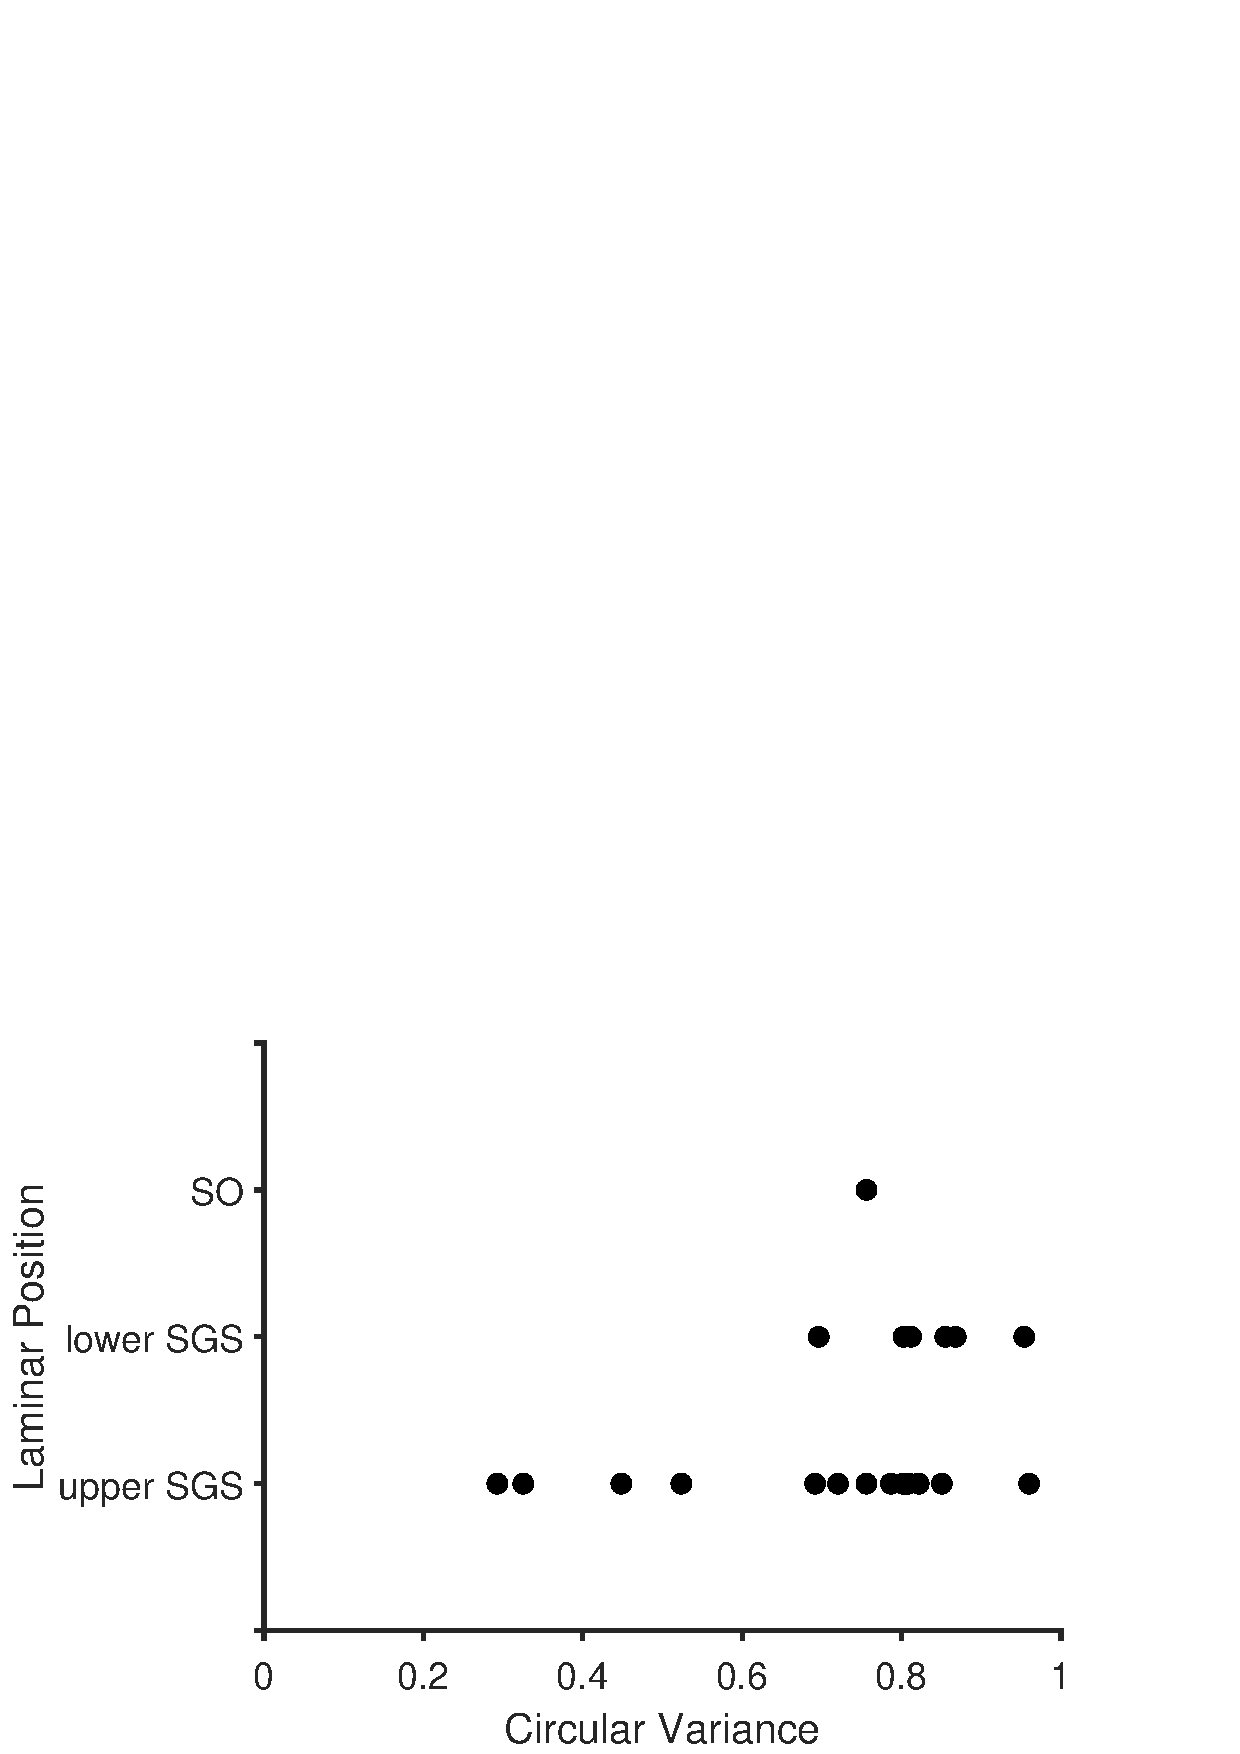
\includegraphics[width=\linewidth]{superiorcolliculus/cvvlampos.jpg}
		\caption{Laminar distribution of the circular variances of the neurons}
		\label{fig:lp}			
	\end{figure}
	
	\subsubsection{Direction selectivity of neurons}
	The distribution of the direction selecitivity index and the DCV of 22 neurons are shown in Figure \ref{fig:ds}a and b. All 22 neurons were included in the analysis as neurons that are not tuned to orientation can be tuned to direction. Figure \ref{fig:dseg}a shows a neuron that is selective to both orientation and direction. \ref{fig:dseg}b shows a neurons selective to direction but not to orientation. The median direction selectivity index was 0.69 (95\% CI= [0.5, 0.83]), suggesting that the majority of the neurons were not direction selective. Of the 22 neurons that were recorded from, only 5 (~20 \%) satisfied our criteria for direction selective neurons. The distribution of the DCV is shown in figure \ref{fig:ds}b. The median DCV was 0.90 (95\% CI= [0.85, 0.93]). The DCV was a more conservative measure of direction selectivity and none of the neurons we measured from were selective to direction.
	
	\begin{figure}[H]
		\includegraphics[width=\linewidth]{superiorcolliculus/directionselectivity_fig.jpg}
		\caption{Distribution of direction selectivity index of 22 superior colliculus neurons using two different measures: the direction selectivity index (a) and the directional circular variance (DCV; b).}
		\label{fig:ds}			
	\end{figure}
	
	\begin{figure}[H]
		\includegraphics[width=\linewidth]{superiorcolliculus/Directionselectivity.jpg}
		\caption{ Example of a cell that is selective to both direction and orientation a) and a cell that is selective to direction but not orientation b).}
		\label{fig:dseg}			
	\end{figure}
	
	\subsubsection{Spatial Frequency Tuning}
	
	A summary of the results of spatial frequency tuning we obtained from 16 neurons is presented in figure \ref{fig:sfcumdist}9a. The median peak spatial frequency was 0.2 cpd (95\% CI= [0, 0.2]) and the median half width at half height was 0.35 cpd (95\% CI= [0.15, 0.55]). Although most neurons reached their peak firing rate quickly, they tended to fire over a range of spatial frequencies as indicated by the slower rise of the high spatial frequency cut off curve. A significant proportion (80\%) of superior colliculus neurons in our sample were also low-pass tuned to spatial frequency (12/16, p= 0.028).
	
	\begin{figure}[]
		\includegraphics[width=\linewidth]{superiorcolliculus/cumsum_sf_SC_LGN.jpg}
		\caption{ Cumulative sum of the low-cutoff, optimum and high cut off spatial frequencies in the tree shrew Superior Colliculus for 16 neurons (a) and the Lateral Geniculate Nucleus for 30 neurons (b; LGN). The LGN results were published in the paper by Van Hooser et al., 2013 and the right side panel is from figure 7b, plotted on the same scale as the SC data in the left hand side panel.}
		\label{fig:sfcumdist}			
	\end{figure}
	
	In order to enable a direct comparison between the superior colliculus and the lateral geniculate nucleus, data from the LGN (from Van Hooser et al., 2013, Figure 7b, 30 neurons) is plotted next to the superior colliculus data (Figure 7b). LGN cells tended to have a higher peak spatial frequencies and lower high frequency cut-offs. However, a similar proportion of neurons are bandpass tuned when compared to the superior colliculus (80\% in the SC vs 76\% in the LGN).
	
	\subsubsection{Orientation tuning using gratings}
	
	The circular variance of the orientation response of eleven neurons was calculated at the peak spatial frequency and compared with those of previously published data in the geniculostriate system of the tree shrews. The distribution of these circular variances are shown in figure \ref{fig:CVvanhooser}. The median CV was 0.84 (95\% CI= [0.77 0.91]). The distribution of the CVs of the superior colliculus and the LGN were similar. While in the LGN nearly 50\% were not tuned to orientation at the peak spatial frequency, only 30\% of the SC neurons did not show orientation tuning (1-CV<0.1). None of the neurons demonstrate sharp orientation tuning (1-CV> 0.5). 
		
	\begin{figure}[]
		\includegraphics[width=\linewidth]{superiorcolliculus/orientation_bias_SG_geniculostriate_2.jpg}
		\caption{ Comparison of the distribution of the orientation selectivity of the LGN, Layer 4 and Layer 2/3 neurons to the distribution of orientation selectivity of the superior colliculus neurons. Horizontal dotted line indicates the 50\% of neurons and the vertical dotted line is the orientation tuning cut off.}
		\label{fig:CVvanhooser}			
	\end{figure}
	
	As there was only enough data in 11 neurons to enable circular variance calculations, the orientation selectivity index (OSI) was calculated for the 16 neurons where gratings of both optimum and orthogonal orientation were shown. The relationship of the OSI and the CV is shown in figure \ref{fig:CVvOSI}. 
	
		\begin{figure}[]
		\includegraphics[width=\linewidth]{superiorcolliculus/CVvsOSI.jpg}
		\caption{Relationship between the circular variance and orientation selectivity index.}
		\label{fig:CVvOSI}			
	\end{figure}
	
	Levick and Thibos (1982) calculated the circular variance of the neurons in their study at different spatial frequencies and found that neurons showed sharper tuning at spatial frequencies higher than the optimum spatial frequency. Since the circular variance and orientation selectivity index show a strong correlation (r= 0.87, p<0.005, n=11), here OSI is used to conduct a similar analysis.
	
	\subsubsection{Relationship between spatial frequency and orientation tuning.}
	When the spatial frequency tuning response of the neuron at different orientations was observed, 13 of 16 neurons were tuned to orientation at higher spatial frequencies. The F0 component of a neuron’s response to gratings of increasing spatial frequencies at the optimum and the orthogonal orientations is shown in figure \ref{fig:scoptorth}. The gray shaded area represents the spatial frequencies where the neuron still responds to gratings of the optimum orientation but no longer responds when gratings of the orthogonal orientation are presented (i.e., the neuron is orientation tuned). The upper limit of the gray shaded area (the dotted line to the right) is the cut off spatial frequency at the optimum orientation. The spatial frequency corresponding to the lower limit of the shaded gray area is the cut off spatial frequency at the orthogonal orientation. The difference in response between the optimum and non-optimum orientation cut off frequencies was calculated. These results for the group are presented in figure \ref{fig:sf_bw}. A one tailed Wilcoxon Signed Rank test showed that the spatial frequency cutoff at the optimum orientation was significantly higher than the spatial frequency cutoff at the orthogonal orientation (median difference= 0.4 cpd; z=3.15; p=0.0008). The magenta circles in figure \ref{fig:sf_bw} show the peak spatial frequency of the respective neuron. The green circles indicate the spatial frequency where the neuron was most tuned to orientation (where the OSI was maximum). The spatial frequency where the orientation tuning of the neuron was greatest was significantly higher than the peak spatial frequency of the neuron (One-tail Wilcoxon Signed Rank test; z=3.3096; p=0.0005), indicating that orientation tuning was only observed at higher spatial frequencies in the tree shrew Superior Colliculus.
	
		\begin{figure}[H]
		\includegraphics[width=\linewidth]{superiorcolliculus/sf_bandwidth.jpg}
		\caption{The difference between the cut-off frequencies for the optimum and orthogonal orientations for 16 units is shown in the above figure. The purple circles are the peak spatial frequencies of the respective neurons and the green circles are the spatial frequency where the cell is most tuned to orientation. In most cases, the neurons are most tuned for orientation at spatial frequencies well past the peak spatial frequency.}
		\label{fig:sf_bw}			
		\end{figure}
	
	\subsubsection{Modulation Index of the neurons.}
	
	For the 16 units whose spatial frequency tuning were recorded, the distribution of modulation ratios is presented in figure 14. A modulation ratio less than one means that the modulated component of the response was lower than the unmodulated component (linear cells) while a modulation ratio of greater than 1 indicates that the respective neurons were non-linear. Most neurons in our sample showed non-linear summation over their receptive fields (Modulation index less than 1). 
	
	\begin{figure}[H]
		\includegraphics[width=\linewidth]{superiorcolliculus/modulation_index.jpg}
		\caption{The distribution of modulation indices of the neurons in our sample. Most neurons had a modulation index less than 1.}
		\label{fig:sc_mi}			
	\end{figure}
	\pagebreak
	\section{Discussion}
	Our results show that majority of the neurons in the superficial layers of the tree shrew superior colliculus show orientation biases when tested with thin bar stimuli. When shown grating stimuli, most neurons also showed low pass spatial frequency tuning and were tuned for orientations at higher spatial frequencies. We also found that a small proportion of neurons were tuned to direction and majority of the neurons showed non-linear summation over their receptive fields.
	
	We used bars to study the orientation selectivity of neurons in the superior colliculus and found that most units (90\%) were biased for orientation. We calculated two measures of orientation selectivity the circular variance and bias. The bias was the ratio of the response at the optimum orientation divided by the response at the orientation orthogonal to the optimum orientation. Neurons with a bias greater than or equal to 3 were comparable to the elongated receptive field units reported by Albano and colleagues. Six out of twenty-two neurons (27 \%) had a bias greater than 3. This is comparable to the proportion of elongated receptive field units (19\%) that were reported by Albano et al (1978). Most of the elongated receptive field units reported by Albano et al (1978) were found in the lSGS and SO layers and none were recorded from the uSGS. In our sample, most neurons were biased for orientation to some degree and neurons that had a bias greater than 3 were found in both the upper and lower SGS with the sharpest tuned neurons found in the uSGS. We only recorded from one neuron in the SO which had a bias value of 2.85. This discrepancy in the detection of orientation biased neurons in the uSGS may be due to the thickness of the bar stimulus used.
	
	Neurons in the subcortical areas show more tuned responses when shown thinner bars (Vidyasagar and Urbas, 1982). This is in line with sub-cortical neurons being tuned to orientation at higher spatial frequencies (Levick \& Thibos, 1980; Levick \& Thibos, 1982). In response to gratings, as in cat and macaque retinal and LGN neurons, at the peak spatial frequency, the SC neurons showed minimal orientation biases. The orientation tuning of a neuron peaked at spatial frequencies greater than the optimum spatial frequency of the neuron in most cases. As a result, if Albano et al., had used thicker bars than we have, they may have found neurons that had elongated receptive fields even in the uSGS.
	
	When the spatial frequency tuning of SC neurons and the LGN neurons in the tree shrew were compared, both LGN and SC neurons showed low pass spatial frequency tuning. However, when compared to the LGN neurons (as published in Van Hooser et al., 2013), the peak spatial frequencies we observed were lower. This could be related to the type of neurons the SC neurons get their inputs from. SC neurons in most species receive inputs from achromatic Y-like or W-like cells (DeMonasterio, 1978; Shapley \& Perry, 1986; Schiller \& Malpeli, 1977; Bunt et al., 1975; Leventhal et al., 1981) These cells show non-linear summation over their receptive fields and tend to have lower peak spatial frequencies (Enroth-Cugell \& Robson, 1966; Derrington \& Fuchs, 1979; So \& Shapley, 1981). The LGN neurons tended to show more modulated responses, typical of X-like neurons (Van Hooser et al., 2013) and as the SC neurons in this study showed non-linear summation (as Y and W like cells do) over their receptive fields, this could explain the difference in the peak spatial frequency tuning. One other difference between the LGN and the SC spatial frequency tuning curves was the high spatial frequency cut-offs. The SC neurons generally tended to have higher spatial frequency cut-offs compared to the LGN neurons. A possible reason for this difference could be the optics. In our study, we carefully tested the responses of the neurons to stimuli of different spatial frequencies to ensure that the animal could resolve gratings of higher spatial frequencies. If uncorrected refractive errors were present in the tree shrews in the study by Van Hooser and colleagues, so that they could not resolve gratings of higher spatial frequencies, then this could explain the difference in the high cut-off values reported between the LGN and the SC.
	
	Most neurons in the tree shrew superior colliculus were not tuned to direction. Van Hooser et al reported that only one neuron in their entire sample was tuned to direction using the DCV. Using the same measure, we found that none of our neurons exhibited direction selectivity. A larger sample may show a small proportion of neurons being tuned for direction using the DCV in the superior colliculus. In their study, Albano and colleagues reported that a proportion of the elongated receptive field cells were also selective to directions and that these cells were found in the lSGS and the SO. However, the proportion of neurons tuned to direction was not reported. Using a less conservative measure than the DCV, the DSI, we found that approximately 20\% of the neurons were tuned to direction. Of the 5 direction selective neurons, 2 were from the uSGS (13\% of the uSGS neurons) and 3 were from the lSGS (50\% of the lSGS neuons) suggesting that direction selective neurons were sparser in the uSGS when compared to the lSGS.
	
	In their study, Albano et al., (1978) proposed that the uSGS and the lSGS could play different functional roles. They found that the uSGS neurons were composed of only one type of neuron (the stationary –responsive type) while the lSGS consisted of a combination of different type of neurons. This claim was supported by anatomical and morpjological evidence; namely, uSGS neurons were generally smaller (5-8 μm) and received predominantly retinal inputs lSGS neurons were larger (8-12 μm) and received inputs from both the retina and the cortex (Abplanalp, 1971). A later study however showed that the retinal inputs dominated the SGS of the tree shrews with the uSGS receiving lesser cortical inputs than the lower SGS. (Graham \& Casagrande, 1980). We found that the uSGS contained the sharpest tuned neurons in our sample and a smaller proportion of these neurons were tuned to direction whereas, all the neurons in the lSGS were broadly tuned to orientation and a higher proportion of neurons were tuned to direction. When compared to Albano et al., we found more diverse response properties in the uSGS rather than the lSGS (e.g.: see figure 6). However, our sample size was small (15 uSGS and 6 uSGS neurons) and any differences we found could be due to sampling differences.
	
	\section{Conclusion}
	In this study we found that neurons in the superior colliculus were tuned to orientation at higher frequencies. Most neurons were low pass tuned to spatial frequency and at the peak spatial frequency, a similar proportion of neurons were biased for orientation in the LGN as well as the SC. In the SC, neurons were sharply tuned to orientation at higher spatial frequencies. This result is consistent with that observed in the retina and the LGN of cats and macaques. Layer 4 neurons of the tree shrews, which resemble LGN neurons (Van Hooser et al., 2013), also respond similarly at higher spatial frequencies (See Tree Shrew Chapter). This similarity in subcortical orientation response across both the geniculo-striate system as well as the SC indicates that orientation biases are present in the tree shrew retina. In the tree shrew, sharp orientation tuning observed in the supra-granular layers could be due to the sharpening of orientation biases by cortical inhibition rather than through Hubel and Wiesel like excitatory convergence as has been proposed (Chisum et al., 2003; Mooser et al., 2004).
	
\chapter{Relationship between orientation tuning and spatial frequency tuning in the tree shrew V1}
\pagebreak
\section{Summary}
\pagebreak
\section{Introduction}

Early studies conducted in the tree shrew primary visual cortex indicated that orientation tuning in the V1 of tree shrews may be generated from excitatory convergence of unoriented, layer 4 neurons onto layer 2/3 neurons. However, the authors acknowledged that while this excitatory convergence is capable of providing orientation biases, the extensive horizontal connections present in the superficial layers of the tree shrew play an important role in sharpening these orientation biases (Chisum et al., 2003; Mooser et al., 2004). Later however, it was shown that layer 4 neurons did not have circular receptive fields as was originally thought but had broad orientation biases (Van Hooser et al., 2013). A separate study by Veit et al (2014) also argued that horizontal connections in tree shrews are important as just the orientation tuning of inputs seemed insufficient to predict the degree of orientation selectivity of the layer 2/3 cells.
Huang et al (2014) when they tried to test how the horizontal connections worked, didn’t really find what they had hoped. Found that horizontal connections contributed linearly to cell responses regardless of the orientations of where the horizontal connection terminated. They also did not find any axial effects as has been predicted in the past. Issues- they  could just be stimulating within 500 microns, where horizontal connections are not specific? Recurrent excitation? Also they could selectively activate only excitatory neurons using their viral vectors which could leave and inhibitory modulatory circuits out.
Recently, using two photon calcium imaging, Lee et al, 2016, suggested that off inputs to the cortex are established by on inputs organising themselves around off inputs which establish topography. However, there are a few caveats to this model. Muly and Fitzpatrick (1992) showed that on and off inputs to layer 2/3 cells have significant overlap. Further, Veit et al (2014) showed that only 7\% of all cells in the shrew V1 had segregated receptive field sub-divisions, lacking the basic RF structure for the majority of the cells to develop orientation selectivity using this method. 



\section{Methods}


\subsection{Surgery and Anaesthesia}

The following surgical procedures were performed on the tree shrews from whom data were collected for chapters 5 and 6. Surgical procedures are as outlined in the Methods chapter. Briefly, the animal was anaesthetized using a mixture of Ketamine and Xylazine, a venous catheter was inserted in to the femoral vein and a tracheostomy performed to assist in breathing during the experiment. The animal was administered muscle paralysant (Vecuronium Bromide) intravenously and was anaesthetised using Isoflurane (0.5-1\%) for the duration of the experiment. Hard contact lenses were fitted to the eye to prevent corneal drying. In some tree shrews, additional lenses were used to correct for any refractive errors. A craniotomy and durotomy were performed over the location of V1 (Horsley-Clarke Co-ordinates A2.5 to P2.5). ECG and frontal EEG were monitored during the experiment. At the end of the experiment, the animal was euthanized using an overdose of pentobarbital sodium and perfused using 0.1M Phosphate Buffer (PB) solution followed by 4\% Paraformaldehyde in 0.1M PB. The brain was removed and stored in sucrose (20-25\%) for histology.

	\subsubsection{Electrophysiology}
High impedence, lacquer coated tungsten microelectrodes (FHC Metal Microelectrodes Inc., ME, USA; impedance= 12-18 MΩ) were lowered into the brain at an angle perpendicular to the cortical surface. The signal was amplified and filtered (x 10,000 gain, bandpass filtered between 300-3000 Hz, A-M systems) and fed into an audio speaker as well as an analog to digital converter (Cambridge Electronic Design Limited, Cambridge, UK; digitised at 22.5 kHz). Neurons were recorded from Layers 2/3 and Layer 4. Layer 4 could be identified by a characteristic ‘swish’, first for on stimuli and then for off stimuli, in the tree shrews. Where we no longer heard the swish, we concluded that we exited layer 4 and into layer 5. Neurons in layers 5 and 6 were not recorded from. Lesions (6 μA for 6s) were made at the end of each track. The electrode was withdrawn and lesions were made at regular intervals to trace the path of the electrode through the brain. The data was recorded as a spike trace using the spike 2 software (CED, Cambridge, UK). The spikes were templated and the spike timing exported as a text file. Further analysis was performed using custom MATLAB code (The Mathworks Inc, USA).
\subsubsection{Stimuli}
A hand-held projectoscope was used to mark the receptive field boundaries. Using this, the centre of the monitor was aligned with centre of the receptive field prior to stimulus presentation. Stimuli were presented using a BARCO monitor (Frame Refresh Rate= 80 Hz; Reference Calibrator Plus; Barco Video and Communications, Belgium) and generated using Visage (VSG, Cambridge Research Systems, Cambridge, UK) and custom Stimulus Description Language (SDL) scripts. The monitor had a mean luminance of 32.6 cdm-2. While recording, the monitor was placed at a distance of 114 cm from the eye. For each of the different stimuli described below, ten complete stimulus presentations were completed.
\paragraph{Bar Stimuli}
For each neurons, an initial estimate of optimum orientation was obtained using bars, moving bi-directionally across the screen. The background was a uniform gray screen. Depending on the polarity of the neurons, either a bright bar or a dark bar was used (contrast= 100 \%). The bar was usually 8$^o$o long (ranging between 4 and 8 degrees) and 0.5$^o$ wide (ranging between 0.1 and 1 degree). A total of 18 different orientations were tested and PSTHs (see chapter 2) were made online using the Spike 2 software. The orientation that yielded the highest firing rate was used for further testing.

\paragraph{Grating Stimuli}
For all neurons, once optimum orientation was determined, spatial frequency tuning of the neurons were studied. Drifting sine-wave gratings (TF= 4Hz, Contrast=100\%) of increasing spatial frequencies (between 0 and 2.2 cpd) and in the optimum orientation were presented to neurons. Further, the spatial frequency response of the neuron to gratings tuned to the orientation orthogonal to the optimum orientation were also recorded. The responses were recorded and stored for further analysis.

\subsubsection{Data Analysis}

\paragraph{Orientation Selectivity of bars}

The orientation selectivity of all the cortical neurons we encountered were measured using thin bars. The circular mean and circular variance of this response was calculated using the following formulas to measure the optimum orientation and sharpness of the tuning.

Circular mean=

Circular Variance=

One of the key predictions of our model was that the optimum orientation of the neuronal response does not vary along a penetration perpendicular to the cortical surface. In order to check this, we calculated the absolute difference in preferred orientation between the first neurons we encounter in layer 2/3 in each track and all the neurons that are present in the same track.

While making electrode tracks, due to the angle of the skull and the brain, it is possible that in some of our penetrations, the electrode angle was not always exactly perpendicular to the skull. In order to make sure that any differences we observed were not due to the angle of the track, we also undertook a simulation. We obtained an orientation tuning map in the tree shrews (Bosking et al., 1997) and 
\subsubsection{Histology and Track Reconstruction}


\section{Results}

\subsubsection{Laminar Position of neurons}

The laminar position of all units were determined using track reconstructions   
\section{Discussion}
\section{Conclusion}

%	\input{summarych}
%	\input{roleofin}
\chapter{Is the tree shrew primary visual cortex a linear filter?}
	\section{Introduction}
	\section{Methods}
		Data from xxx neurons in xxx animals are presented here. Briefly, the animals were anaesthetised and surgery was performed in the manner described in section -link methods chapter here-. An electrode was inserted into the primary visual cortex of the anaesthetised tree shrew and electrophysiological recordings were performed in the manner described in section- link methods chapter here-. The stimuli presented and the data analysis performed are described below.
		
			\subsection{Stimuli}
				All stimuli were presented on a Barco monitor and stimuli were generated using the SDL (Visage system). The responses of each neuron to the following stimuli were measured. First, the orientation tuning of the neurons was measured by presenting thin moving bars of different orientations. Each orientation was presented 10 times and bars of 9 different orientation moving in two directions were presented. The orientation for which the neuron gave the maximum response was taken as the optimum orientation. Following this, drifting gratings of increasing spatial frequencies were presented in the optimum orientation. The responses of the neurons were recorded. In some cases (number), light and dark bars of the optimum orientation were also presented\cite{Chisum2003a}.
				
			\subsection{Data Analysis}
				All neuronal responses were first carefully templated to only include the data from one neuron. A spike density function was calculated as described in the --methods--. This was used for further analysis.
				
				\subsubsection{Classifying neurons using grating responses}
					
					
					The spike density function of the moving grating response was analysed using a fourier transform. The first fundametal response (F1) was calculated as the peak in the frequency domain corresponding to the temporal frequency at which the grating drifted. The F0 component of the response was taken as the response at 0Hz. The F0 and F1 response for all neurons were calculated. 
					
					\paragraph{The F1/F0 ratio}
					
					Simple cells have a modulated response to the light and the dark regions of a drifting grating. For example, in an on simple cell, the leaving of the dark region of the grating and the presentation of a light region to the neuron evokes a strong response while the opposite suppresses response. The F1 component of the response capitulates this modulated response. Complex cells on the other hand respond uniformly to both the dark and light regions of the grating and as a result, a simple average of the response accurately reflects the response fo the neuron. The F1/F0 ratio (proposed by Skottun et al., 1987) accurately distinguishes between simple and complex cells. A simple cell will have a significantly higher modulated response compared to the unmodulated response. Therefore, a cell is classified as simple if the F1:F0 ratio is greater than 1.5. A cell is classified as complex if the F1:F0 ratio is less than 1. Neurons with F1/F0 ratio between 1 and 1.5 may be A cells described by Henry et al.,1977.
					 
				\subsubsection{Classifying neurons using bar responses}
					According to Hubel and Wiesel (1962), neurons in the primarv visual cortex could be either simple, complex or hypercomplex cells. Simple cells received mostly first order inputs from the LGN and consisted of separate on and off subregions. Complex and hypercomplex cells were higher order cells and had overlapping on and off regions. The responses obtained with moving dark and light bars were used to test if neurons had segregated on and off regions. This was done by overlaying the spike density functions of the on and off responses. A segregation index was also calculated as described below.
					
					\paragraph{Segregation Index (SI)}
					
					The spontaneous activity, calculated as the response to a 'blank' screen, was measured. This response was then subtracted from the response of the neuron to both light and dark bars to accurately determine the response to the stimulus at each time point. The segregation index was then calculated using the following formula.
					\[SI= \frac{\sum(Off Response_t- On Response_t)}{\sum(Off Response_t+ On Response_t)}\]
					
					
					The value of SI thus calculated will range from 0 to 1. A neuron that has an SI of 1 will be a simple cell and a neuron with SI closer to 0 will be a complex cell. Where both grating and bar data were available for a neuron, the F1/F0 modulation ratio was used to classify the neuron and the SI was calculated to verify the classification.
					
				\subsubsection{Spatial Frequency Tuning of a neuron}
					
					The response of a neuron to drifting gratings of different spatial frequencies at the optimum orientation was used to calculate the spatial frequency tuning curve for the neuron. For \textbf{all} neurons, the F1 component of the grating response was used to calculate the spatial frequency tuning curve. Where the F1 component is not greater than 5 spks/s, the neuron was excluded from further analysis.
					
					\paragraph{Peak Spatial Frequency}
					
					The spatial frequency for which the neuron gave the highest modulated response was taken as the peak spatial frequency.
					
					\paragraph{Spatial Frequency Bandwidth}
					
					The bandwidth of the Spatial Frequency tuning curve was calculated as follows. First, a cut off response was identified as half the maximum response. Then the spatial frequencies where the spatial frequency tuning curve first reached the cut-off response before and after the response reached maximum response were identified. The difference of the two spatially frequencies were taken. The log of this difference was also taken to get the spatial frequency bandwidth in octaves.
					
					The peak spatial frequency and the spatial frequency bandwidth of each neuron were then compared.
					
					

	\section{Results}
	
		Spatial frequency tuning data was collected from 68 neurons. Of these units, the maximum modulated response did not exceed 5 spks/s in 6 units. These were excluded from further analysis. The distribution of the F1/F0 ratio are presented below. As expected, there was bimodal distribution, with a peak less than 1 indicating complex cells and one greater than one for simple cells. 
		
			\begin{figure}
				
				\includegraphics[width=\linewidth]{LinearV1/ModulationRatio.jpg}
				\caption{Distribution of modulation ratio}
				\label{fig:fig1}
			\end{figure}
		
		The below table shows the number of cells in the following modulation ratio categories. The majority of the cells we encountered were complex like with the second highest being A cells. Using the modulation ratio, only 14 cells were classified as simple cells.
		
		\begin{table}
			\begin{center}
			\begin{tabular}{ c c c } 
				\hline
				Modulation Ratio & Cell Type & Number of cells \\
				\hline
				Less than 1 & Complex & 28 \\ 
				Between 1 and 1.5 & A & 20 \\ 
				Greater than 1 & Simple & 14 \\ 
				\hline
			\end{tabular}
			\caption{Types of cells in V1}
			\label{table:1}
			\end{center}
		\end{table}
		
		Of the 62 neurons whose data we will be using, 45 also had responses to the moving dark and light bars. A distribution of the segregation indices is shown below.
	\section{Discussion}
%\chapter{Introduction}

\subsubsection{Problems and Objectives of the study}

Neurons in the visual system show feature selectivity; they respond optimally to features of stimuli such as the orientation of the stimulus, the 
Over the years, sub-cortical orientation biases have been shown to play a significant role in  two key areas of study in the primary visual cortex. The first is its role in generating sharp orientation selectivity in the cortex and second is its role in generating the cortical architecture. In my thesis, I aim to further characterise the sub-cortical orientation biases and examine their role in visual processing. In the first part of my thesis, I would like to characterise the origin of the biased sub-cortical input to the cortex. There is debate as to exactly when in visual processing the orientation bias observed in the cortical input is generated. Some studies claim that this orientation bias is generated early on in the visual processing: namely the retina. Some others claim that these biases are generated through a mechanism such as excitatory convergence in the cortex. This part probes this question in two ways. 

\subsubsection{Chapter 6}

This chapter examines if there is a preponderance of a particular orientation in the cortical inputs. If the orientation bias in the cortical input is generated by Hubel and Wiesel type excitatory convergence --- where circular LGN receptive fields converge on to a V1 neuron --- we would expect that inputs to the cortex don't show any preferences (i.e. the orientations of the inputs will be randomly distributed.). Many studies however, have shown that RGCs and LGN neurons are preferentially tuned to the radial orientation (the orientation of the line joining the center of the receptive field to the centre of visual field). If the orientation bias in the inputs is derived from the retina instead, then this 
	
	
%\input{./chapters/02_Theory/Theory.tex}
%\input{./chapters/03_DWI/DWI.tex}
%\input{./chapters/04_Sodium/Sodium.tex}
%\input{./chapters/05_EchoAveraging/EchoAveraging.tex}
%\input{./chapters/06_Conclusion/Conclusion.tex}

%\bibliographystyle{ieeetr}
%\bibliography{./biblio/refs_theory,./biblio/refs_GOLD,./biblio/refs_MLOFI,./biblio/refs_sodium}

\end{document}